\documentclass{article}

% Language setting
% Replace `english' with e.g. `spanish' to change the document language
\usepackage[spanish]{babel}

% Set page size and margins
\usepackage[a4paper,top=2.5cm,bottom=2.5cm,left=3cm,right=3cm,marginparwidth=1.75cm,twoside]{geometry}

% Useful packages
\usepackage{amsmath}
\usepackage{graphicx}
\usepackage{mathtools}
\usepackage[colorlinks=true, allcolors=blue]{hyperref}
\usepackage{indentfirst}                %
\setlength{\parindent}{0.6cm}           % Proper indentation and paragraph spacing
\setlength{\parskip}{0.4cm}             %
\renewcommand{\baselinestretch}{1.3}    %
\usepackage{amsfonts} % for math fonts
\usepackage[table,xcdraw]{xcolor} % for tables and colours
\newcommand{\vect}[1]{\boldsymbol{#1}} % bold and italic vectors
\newcommand{\diff}[0]{\mathrm{d}} % differential
\newcommand{\degree}[0]{^{\circ}}
\usepackage{fancyhdr} % for headings & footers
\usepackage{float} % to maKE THE FREAKING TABLES STAY PUT
\usepackage{physics} % pHysiks
\usepackage[justification=centering]{caption} % centre all captions automatically
\usepackage{xfrac}
\usepackage{lipsum}
\usepackage{graphicx}
\definecolor{light-gray}{gray}{0.95}
\newcommand{\code}[1]{\colorbox{light-gray}{\texttt{#1}}}
\usepackage{minted}

% Footer configuration
\pagestyle{fancy}
\fancyhead{}
\renewcommand{\headrulewidth}{0cm}
\fancyfoot[CO,CE]{}
\fancyfoot[RO,LE]{\color{black!50}\thepage}
\fancyfoot[LO,RE]{\color{black!50}\Title}

% Title and authors
\title{Práctica de control de un motor de corriente continua}
\author{Miguel Quiroga González}
\makeatletter\let\Title\@title\makeatother % to reference the title using \Title
\makeatletter\let\Author\@author\makeatother % to reference the author using \Author

%----------------------TITLE------------------------
\begin{document}
\begin{titlepage}
\begin{center}
    \vspace*{3cm}
    \huge
    \textbf{\Title}
    
    \vspace{0.5cm}
    \normalsize
    Sistemas dinámicos y realimentación
    
    \vspace{1cm}
    \large
    \Author
    
    \vspace{1cm}
    \small
    \color{black!50}
    Grado en Física\\
    \today
    
    \vfill
    
\includegraphics[width=0.4\textwidth]{UCM logo}
    \vspace{2cm}
\thispagestyle{empty}
\end{center}
\end{titlepage}
\newpage \thispagestyle{empty} \newpage
%---------------------------------------------------
%  INTRODUCTION
%---------------------------------------------------

\section{Manejo en lazo abierto}\label{sec:p1}

El motor empleado en esta sección de la práctica es el mismo que se utilizará en las secciones restantes. Lo primero que se realiza con el motor elegido es comprobar su correcto funcionamiento. Esto se consigue mediante su manejo en lazo abierto, sin realimentación de ningún tipo. El modelo de Simulink utilizado para esta función se presenta en las figuras a continuación.

\begin{figure}[H]
    \centering
    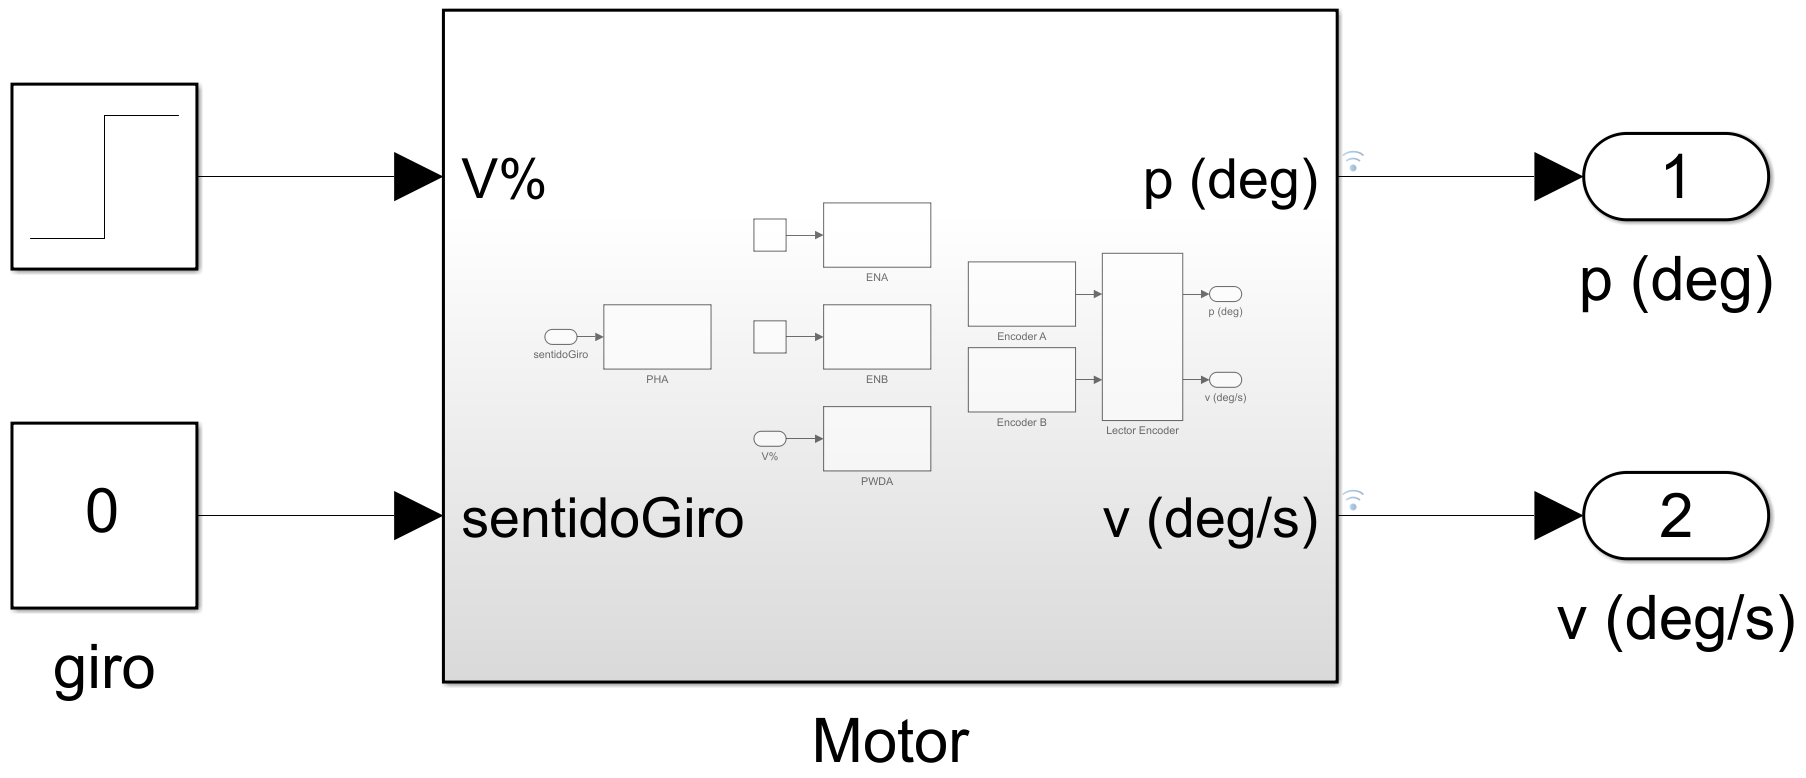
\includegraphics[width=0.75\linewidth]{img/modeloLazoAbierto.png}
    \caption{Superficie del modelo de Simulink para control en lazo abierto.}
    \label{fig:modeloLazoAbierto}
\end{figure}

\begin{figure}[H]
    \centering
    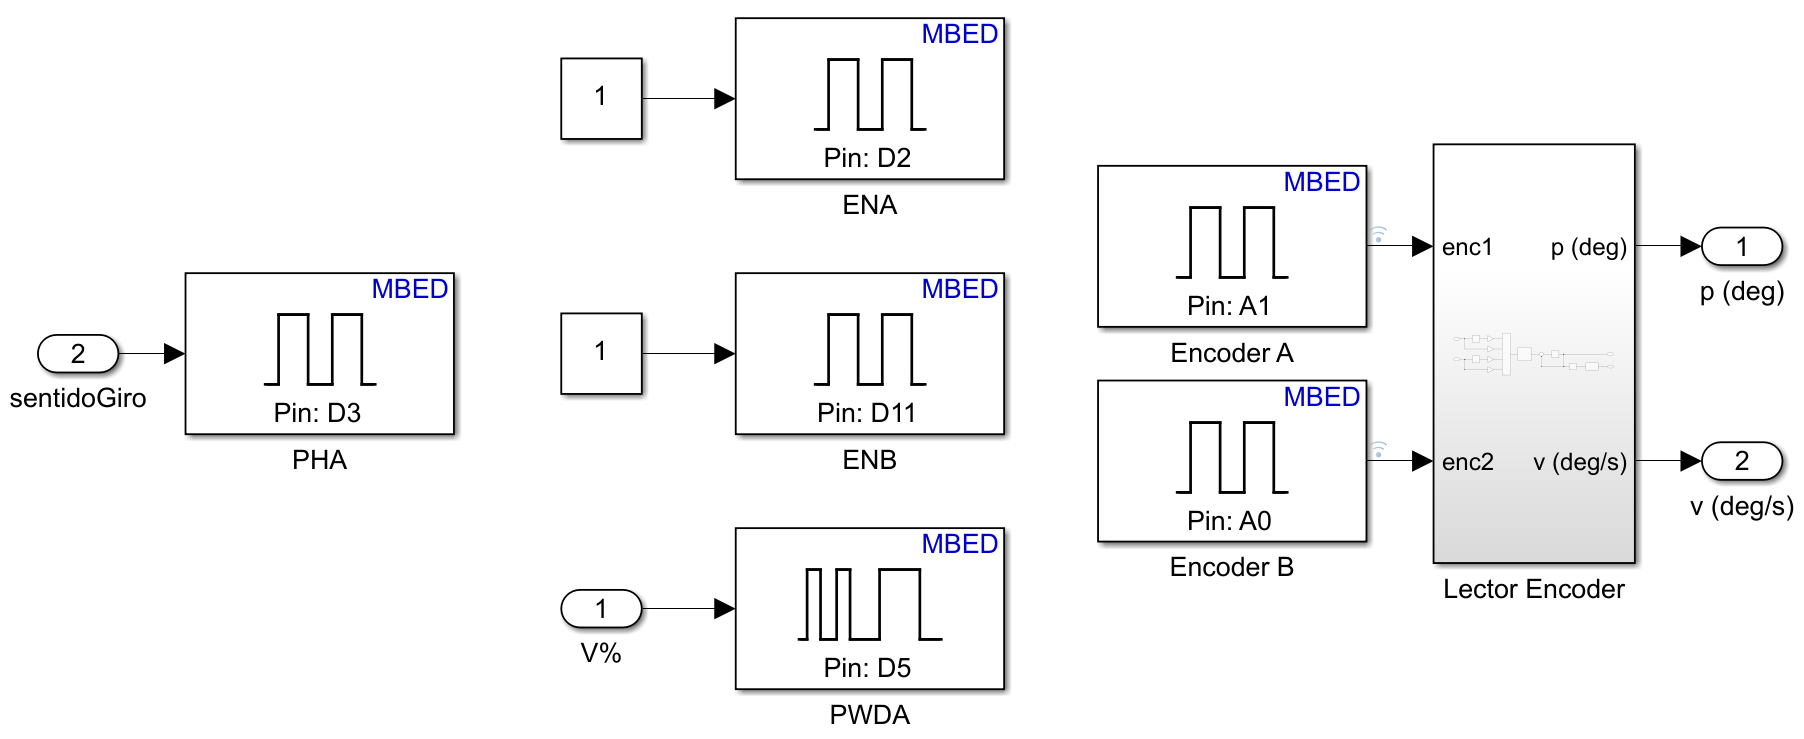
\includegraphics[width=0.75\linewidth]{img/modeloLazoAbiertoPines.png}
    \caption{Dirección de pines y lectura de \textit{encoders}.}
    \label{fig:modeloLazoAbiertoPines}
\end{figure}

\begin{figure}[H]
    \centering
    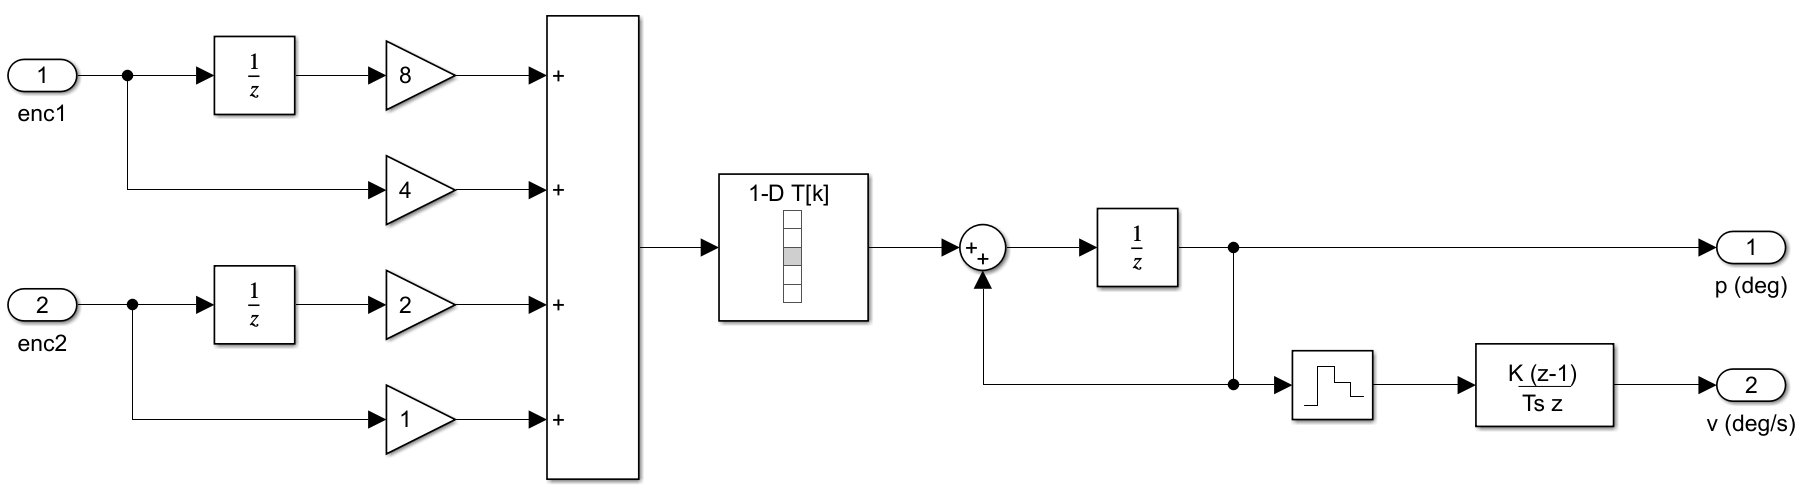
\includegraphics[width=0.75\linewidth]{img/lectorEncoders.png}
    \caption{Lector de los \textit{encoders} del motor.}
    \label{fig:lectorEncoders}
\end{figure}

En este modelo se introduce una señal de escalón a la entrada denominada \code{V\%}, la cual representa el porcentaje de voltaje suministrado al sistema, siendo un 0\% 0 voltios y un 100\% 12 voltios. En las figuras \ref{fig:posicionLazoAbierto} y \ref{fig:velocidadLazoAbierto} se observan los datos tomados de la posición y velocidad del motor, respectivamente. Se puede apreciar como la medida de la posición es predecible, pero la de la velocidad salta continuamente entre dos valores. Esto es debido al método de toma de datos mediante los sensores en cuadratura. Estos únicamente permiten obtener con fiabilidad la posición, por lo que la velocidad se ha de extraer de la misma posición.

\begin{figure}[H]
    \centering
    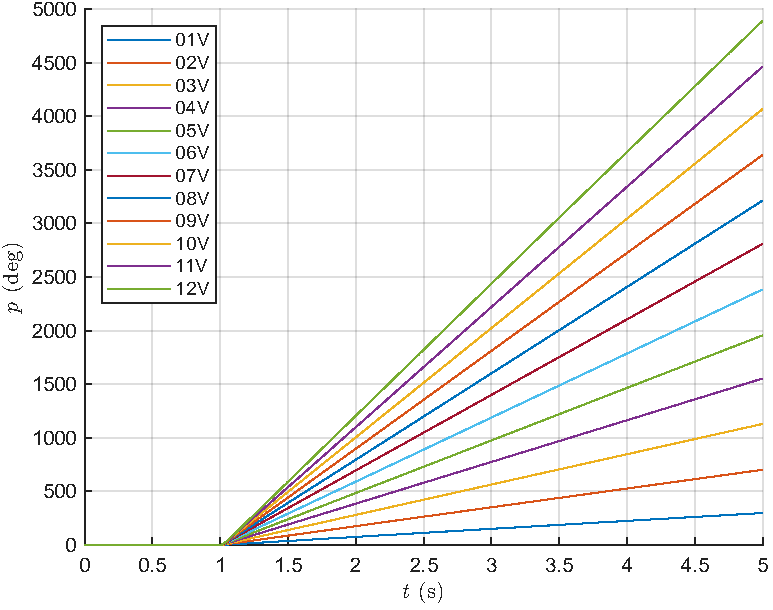
\includegraphics[width=0.75\linewidth]{img/posicionLazoAbierto.pdf}
    \caption{Posición medida según el voltaje.}
    \label{fig:posicionLazoAbierto}
\end{figure}

\begin{figure}[H]
    \centering
    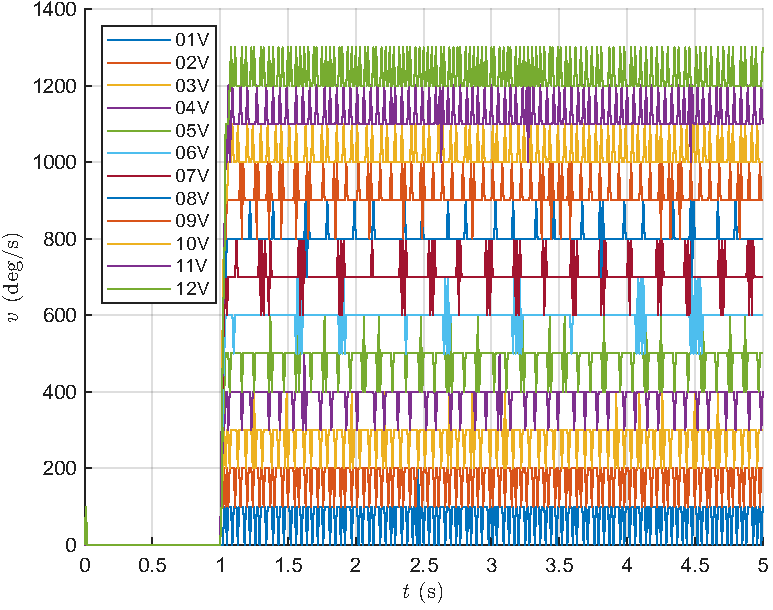
\includegraphics[width=0.75\linewidth]{img/velocidadLazoAbierto.pdf}
    \caption{Velocidad medida según el voltaje.}
    \label{fig:velocidadLazoAbierto}
\end{figure}

Respecto a los sensores en cuadratura, en la figura \ref{fig:encodersCheck} se puede apreciar cómo, incluso a velocidad constante, a veces éstos se saltan medidas. Esto realmente no es un problema muy grave debido a que el sistema evoluciona mucho más rápido que los pulsos individuales de estos encoders. Pese a saltarse algunas medidas, el sistema no sé ve gravemente afectado.

\begin{figure}[H]
    \centering
    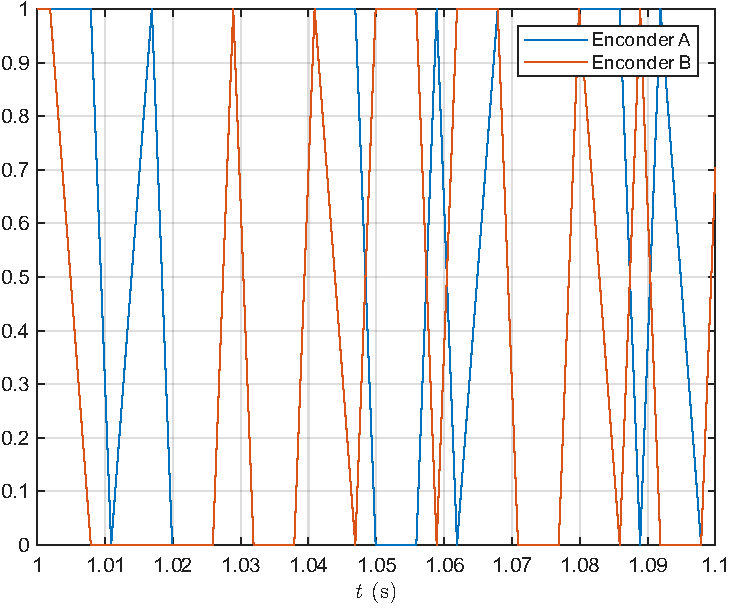
\includegraphics[width=0.75\linewidth]{img/encodersCheck.pdf}
    \caption{Señal de los encoders.}
    \label{fig:encodersCheck}
\end{figure}


\section{Modelado e identificación}

Cuando se aplica una señal de escalón $e(t) = V$ al sistema, la respuesta de la posición angular del mismo es
\begin{equation} \label{eq:angPos}
    \theta(t) = V\frac{k_e}{p^2}\mathrm{e}^{-pt} + V\frac{k_e}{p}t - V\frac{k_e}{p^2},
\end{equation}
y la velocidad angular será por lo tanto
\begin{equation}
    \omega(t) = \dot\theta(t) = -V\frac{k_e}{p}\mathrm{e}^{-pt} + V\frac{k_e}{p}.
\end{equation}

El término con la exponencial corresponde al \textit{wind-up} del motor, es decir, una respuesta no estacionaria. En el caso de este sistema ésta respuesta es muy rápida y se puede eliminar a la hora de ajustar los datos para la identificación del motor. Esto permite realizar un simple ajuste lineal. Además, permite modelar el sistema mediante matrices del siguiente modo:
\begin{align}
    \begin{bmatrix}
    \dot\theta \\
    \dot\omega
    \end{bmatrix} &= \begin{bmatrix}
    0 & 1 \\
    0 &-p
    \end{bmatrix}\cdot\begin{bmatrix}
    \theta \\
    \omega
    \end{bmatrix}+\begin{bmatrix}
    0\\
    k_e
    \end{bmatrix}e(t); \\
    y &= \begin{bmatrix}
    1& 0
    \end{bmatrix}\cdot\begin{bmatrix}
    \theta \\
    \omega
    \end{bmatrix}.
\end{align}

Comparando este sistema con un sistema lineal arbitrario, es evidente que
\begin{equation}\label{eq:ecuacionesSistema}
    A = \begin{bmatrix}
        0 & 1 \\
        0 &-p
    \end{bmatrix};\quad
    B = \begin{bmatrix}
        0\\
        k_e
    \end{bmatrix};\quad
    C = \begin{bmatrix}
        1& 0
    \end{bmatrix};\quad D = 0.
\end{equation}


Una vez se tiene un modelo matemático del comportamiento del sistema, se procede a hacer la identificación del motor empleado en la práctica. Para ello se emplean los datos presentados en las figuras \ref{fig:posicionLazoAbierto} y \ref{fig:velocidadLazoAbierto}. Antes de proceder al ajuste de los datos, se realiza una depuración de los mismos, eliminando el primer segundo de inacción y escogiendo únicamente los primeros dos segundos de operación. Esto evita la incorporación de errores en los parámetros del sistema. Evidentemente también se ignoran los datos de la respuesta a 0 V, puesto que el motor se halla estático.

En la tabla \ref{tab:paramPerVoltage} se presentan los datos obtenidos para cada voltaje tras realizar un ajuste lineal siguiendo la expresión \ref{eq:angPos}.

\begin{table}[H]
\centering
\caption{Valores de los parámetros del sistema}
\label{tab:paramPerVoltage}
\begin{tabular}{ccc}
$V$ (V) & $k_e\cdot10^3$ (deg V$^{-1}$ s$^{-2}$) & $p$ (s$^{-1}$) \\ \hline
1       & 5.2899                                 & 69.9906        \\
2       & 8.3536                                 & 94.6228        \\
3       & 8.3763                                 & 88.7427        \\
4       & 7.9683                                 & 81.8434        \\
5       & 8.2836                                 & 84.5199        \\
6       & 8.7220                                 & 87.6272        \\
7       & 8.1479                                 & 81.0227        \\
8       & 7.8191                                 & 77.6825        \\
9       & 6.9450                                 & 68.5878        \\
10      & 7.1908                                 & 70.6311        \\
11      & 5.6286                                 & 55.3149        \\
12      & 4.9612                                 & 48.3772        
\end{tabular}
\end{table}

Observando los datos de la tabla se puede apreciar como el motor encuentra su respuesta más rápida y precisa para los voltajes medios. Esto es principalmente debido al término $p$, que corresponde al \textit{wind-up} del motor.

Con el objetivo de llegar a un único valor de los parámetros, se realiza una simple media de los valores de la tabla y se consigue que $k_e = 7.3072\cdot10^3$ deg V$^{-1}$ s$^{-2}$ y $p = 75.7469$ s$^{-1}$. Con estos valores, se procede a construir un modelo de Simulink para simular el motor con sus parámetros. Realmente este es un modelo ideal puesto que no tiene en cuenta el \textit{wind-up}.

\begin{figure}[H]
    \centering
    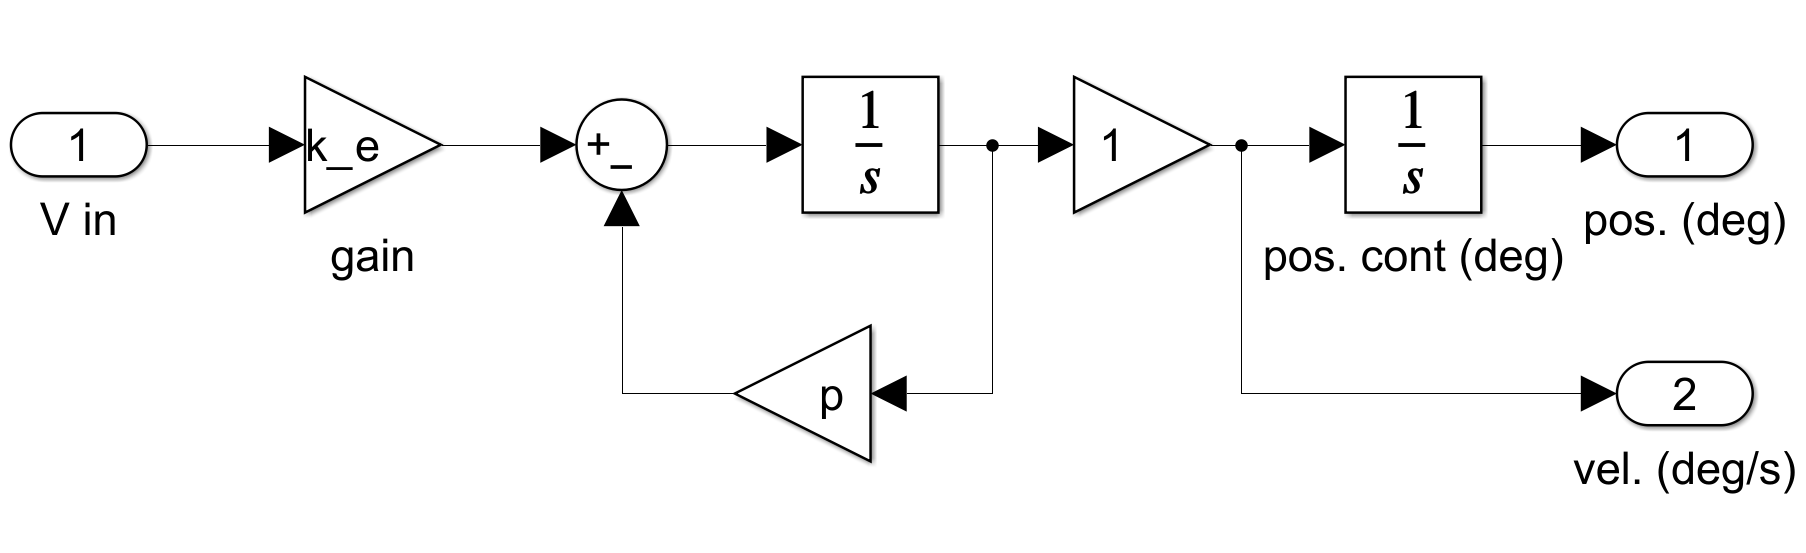
\includegraphics[width=0.75\linewidth]{img/motorIdeal.png}
    \caption{Modelo del motor en Simulink.}
    \label{fig:motorIdeal}
\end{figure}

Simulando este sistema para los mismos voltages que en la sección \ref{sec:p1}, se obtienen resultados similares. Éstos pueden ser vistos en las figuras \ref{fig:posicionIdeal} y \ref{fig:velocidadIdeal}. La diferencia más notable es en las velocidades angulares. Al ser esto una simulación, los datos no se han de extraer de dos sensores en cuadratura, y por lo tanto los resultados son más razonables.

\begin{figure}[H]
    \centering
    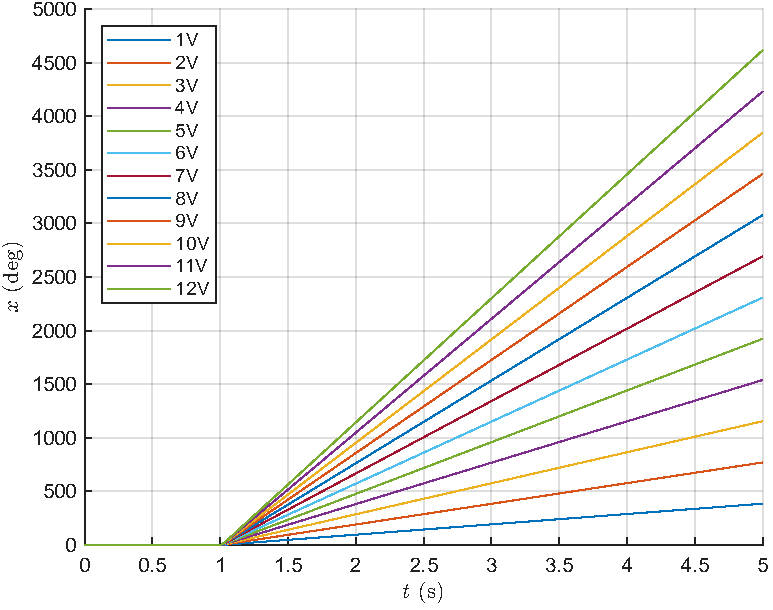
\includegraphics[width=0.75\linewidth]{img/posicionIdeal.pdf}
    \caption{Posición simulada con el modelo ideal.}
    \label{fig:posicionIdeal}
\end{figure}

\begin{figure}[H]
    \centering
    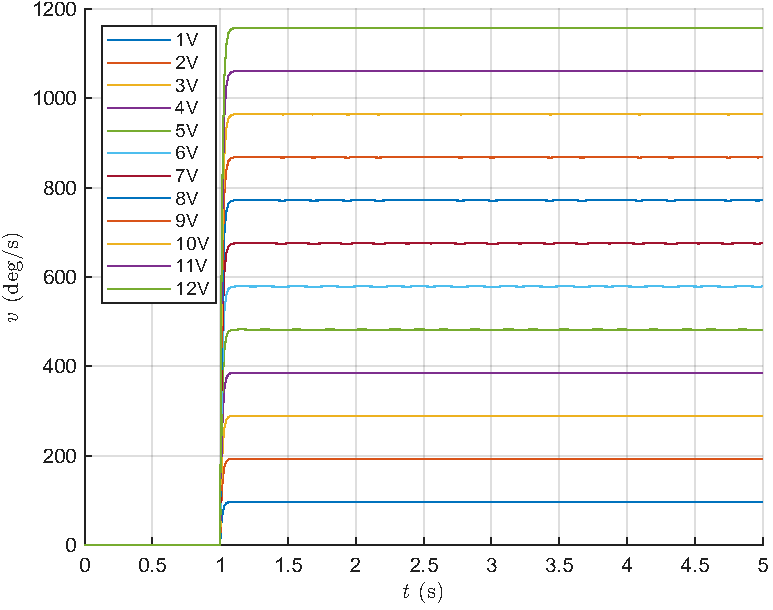
\includegraphics[width=0.75\linewidth]{img/velocidadIdeal.pdf}
    \caption{Velocidad simulada con el modelo ideal.}
    \label{fig:velocidadIdeal}
\end{figure}


\section{Simulación completa del motor}

Con el objetivo de poder simular el motor ideal con el sistema de la figura \ref{fig:motorIdeal}, se han de implementar varios comportamientos que tiene el motor real. Estos son sus \textit{encoders} y el lector correspondiente, así como una alimentación mediante señal PWM. Esto último además deberá incluir el puente H, para poder girar el motor en ambos sentidos. La señal PWM se consigue mediante el circuito de Simulink presentado en la figura \ref{fig:PWM}. El puente H lo componen los bloques que rodean el subsistema PWM en la figura \ref{fig:simIdeal}, que consisten en extraer el signo del valor suministrado y volverlo a aplicar a la señal una vez generada la señal PWM. Adicionalmente se añade un bloque previo de \textit{deadzone} que ignora voltajes menores a 0.5 V.

\begin{figure}[H]
    \centering
    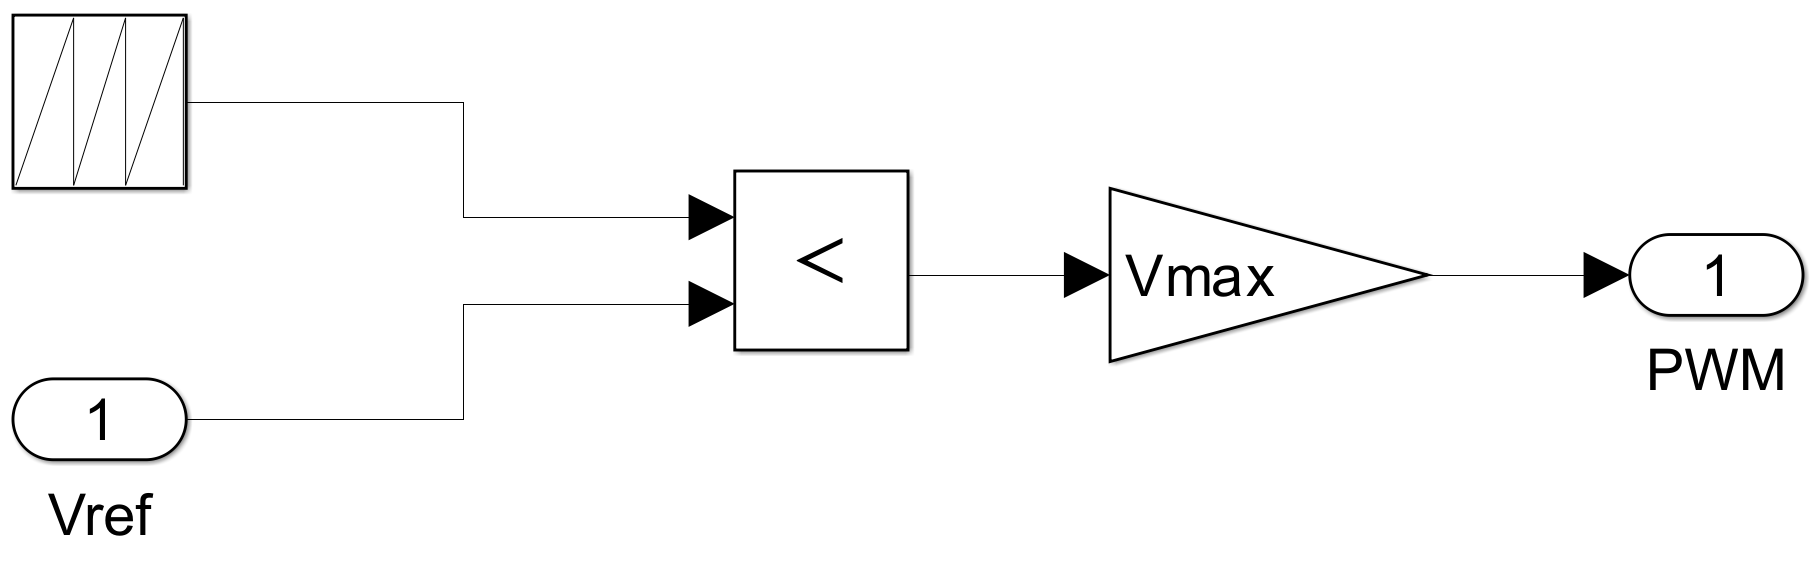
\includegraphics[width=0.75\linewidth]{img/PWM.png}
    \caption{Simulación de la señal PWM.}
    \label{fig:PWM}
\end{figure}

Como se ha mencionado antes, también se necesita un sistema que codifique la posición y velocidad del motor tal y como lo hacen los sensores en cuadratura del motor real. De este modo se podrá usar posteriormente el sistema de la figura \ref{fig:lectorEncoders} para leer los \textit{encoders}. El sistema que realiza esto se encuentra en la figura \ref{fig:encoder}. La ganancia \code{rad2deg} que aparece en el modelo se emplea únicamente si el motor se configura para proveer los valores de posición y velocidad en radianes y radianes por segundo, respectivamente. Al no ser el caso, esta ganancia se deja en 1.

\begin{figure}[H]
    \centering
    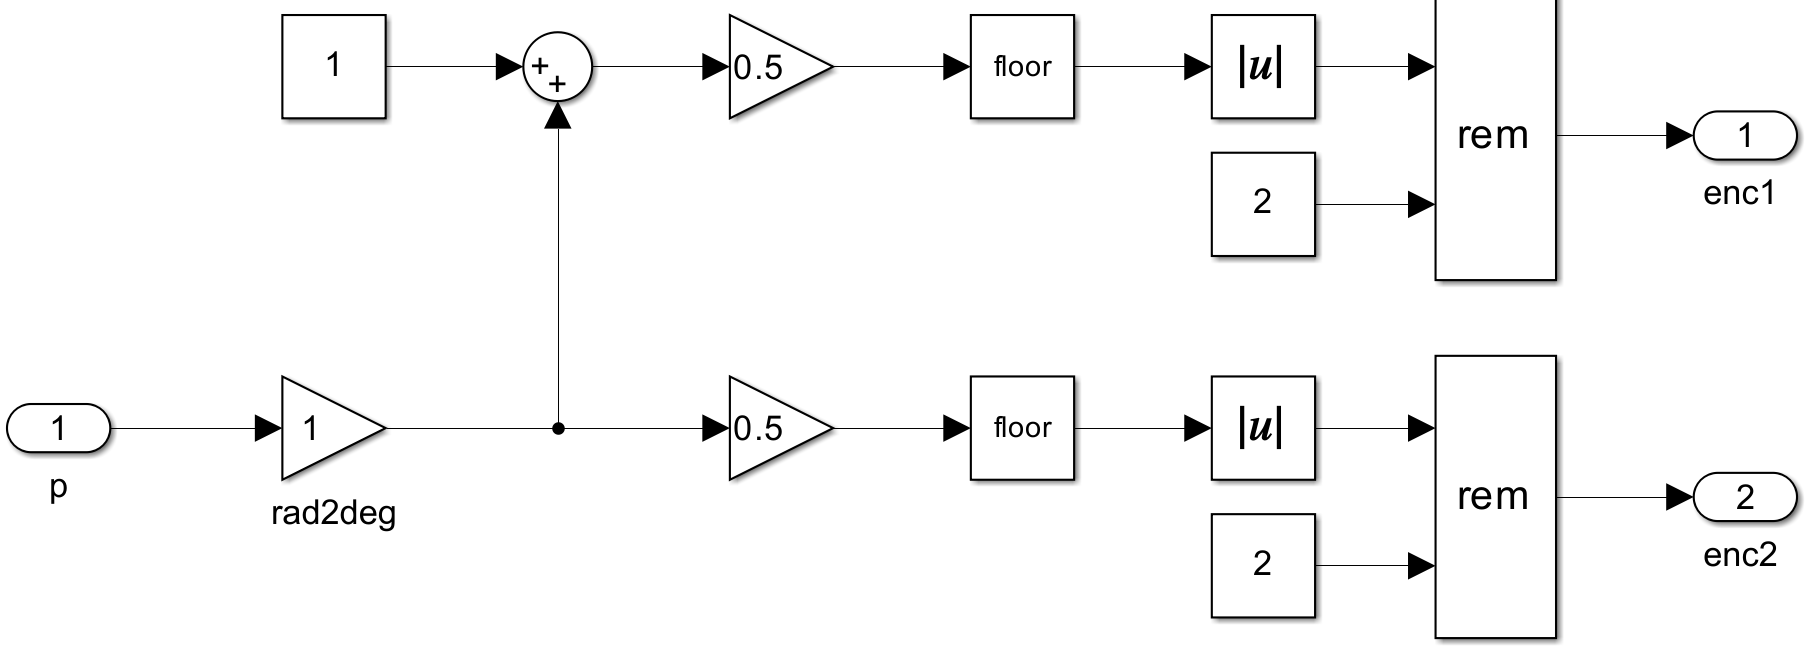
\includegraphics[width=0.75\linewidth]{img/encoder.png}
    \caption{Codificador de las señales del motor para simular sensores en cuadratura.}
    \label{fig:encoder}
\end{figure}

\begin{figure}[H]
    \centering
    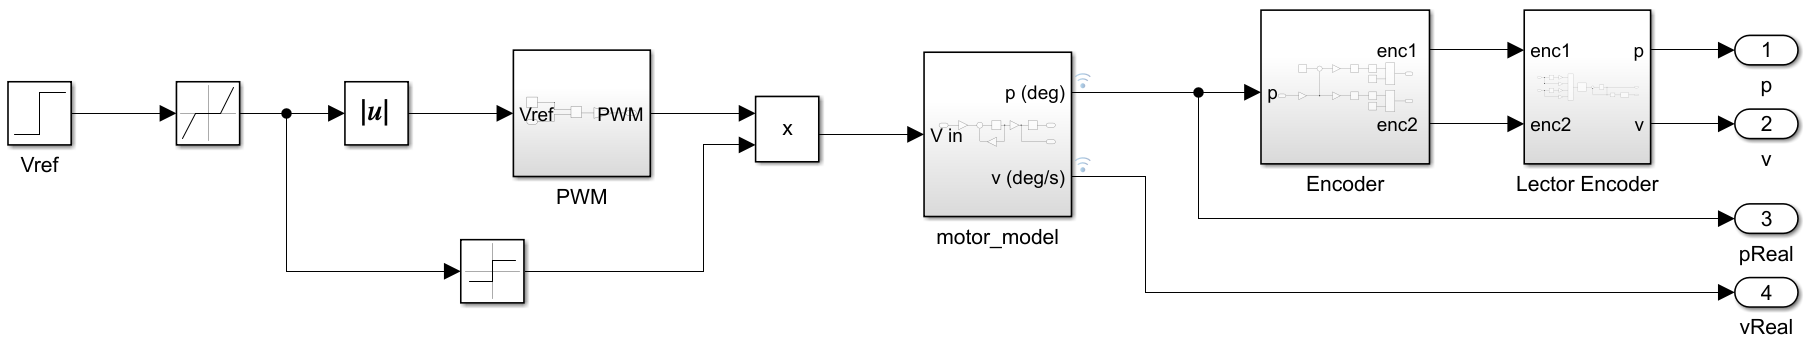
\includegraphics[width=0.75\linewidth]{img/simIdeal.png}
    \caption{Sistema de simulación ideal completo.}
    \label{fig:simIdeal}
\end{figure}

Finalmente se tiene el modelo completo para simular el motor en lazo abierto (fig. \ref{fig:simIdeal}). La primera comprobación a realizar es que los valores de posición y velocidad que proporciona el lector de los \textit{encoders} sean iguales a las posiciones y velocidades reales simuladas. En la figura \ref{fig:comprobacionEncoders} se puede observar como el lector de posición encaja a la perfección con la posición del motor. Sin embargo lo mismo no es cierto para la velocidad, la cual tiene altibajos en torno al valor real que debería tener. Esto es algo que se tendrá en cuenta para próximas secciones de la práctica, puesto que también era un problema con los datos del motor real.

\begin{figure}[H]
    \centering
    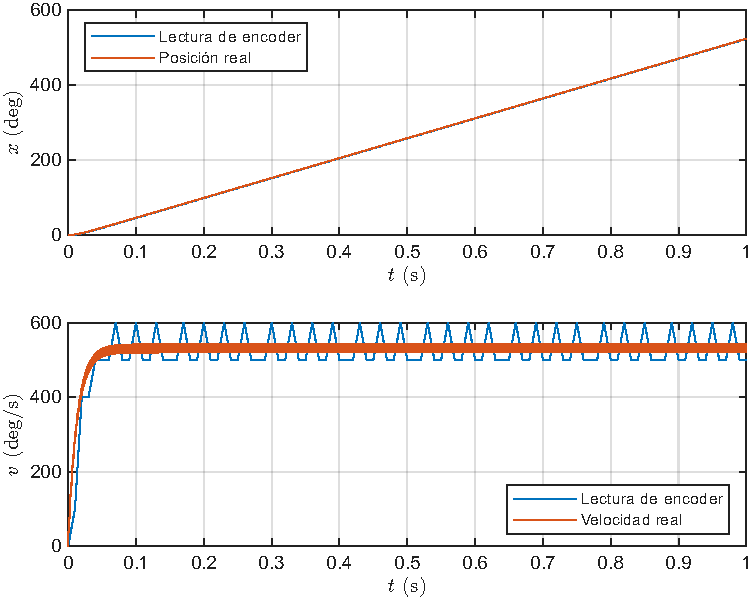
\includegraphics[width=0.75\linewidth]{img/comprobacionEncoders.pdf}
    \caption{Comprobación de la validez del lector de \textit{encoders}.}
    \label{fig:comprobacionEncoders}
\end{figure}

Además, se puede obtener una gráfica con la respuesta del sistema a cada valor de voltaje desde 1 a 12 V aumentando en la unidad (fig. \ref{fig:posicionIdealEncoder} y \ref{fig:velocidadIdealEncoder}), del mismo modo que en las secciones anteriores. Se puede apreciar como la respuesta es similar a las gráficas previas.

\begin{figure}[H]
    \centering
    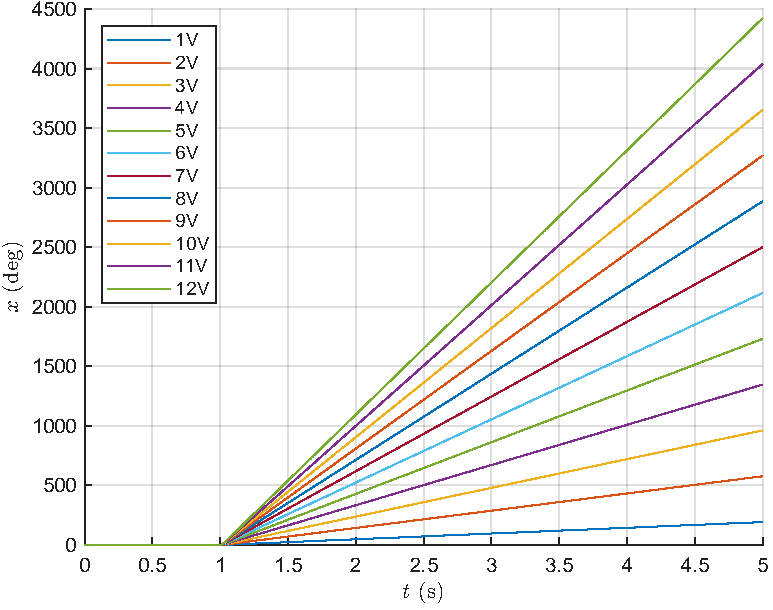
\includegraphics[width=0.75\linewidth]{img/posicionIdealEncoder.pdf}
    \caption{Posición simulada según el \textit{encoder}.}
    \label{fig:posicionIdealEncoder}
\end{figure}

\begin{figure}[H]
    \centering
    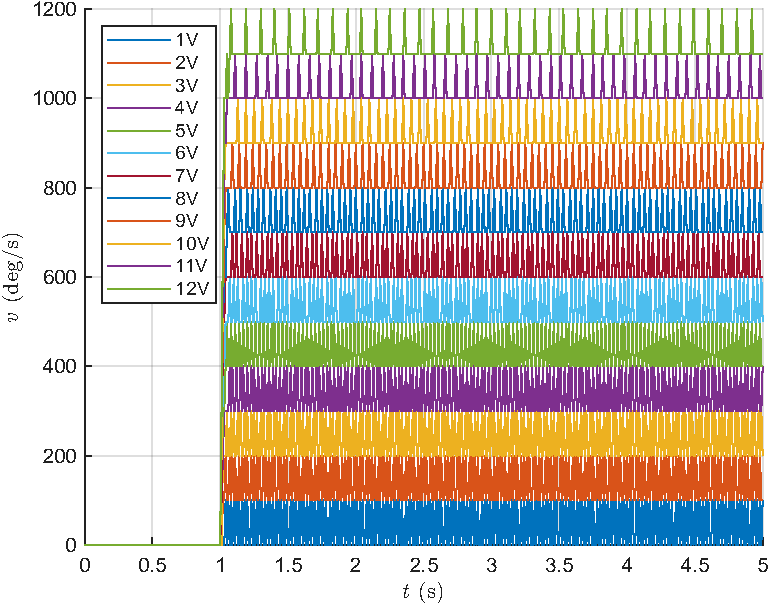
\includegraphics[width=0.75\linewidth]{img/velocidadIdealEncoder.pdf}
    \caption{Posición simulada según el \textit{encoder}.}
    \label{fig:velocidadIdealEncoder}
\end{figure}


\section{Diseño de un controlador por realimentación de estados estimados}

Volviendo al motor ideal sin imitar su comportamiento real, se va a diseñar un sistema que permita controlar el motor y llevarlo a una posición de consigna elegida. Esto se hará mediante una realimentación de estados y un control integral. Sin embargo, como se explicó previamente, los datos de la velocidad del motor no son de fiar, por lo que también se empleará un estimador de estados. Es por esto que en la ecuación \ref{eq:ecuacionesSistema} se eligió ese valor para $C$.

\begin{figure}[H]
    \centering
    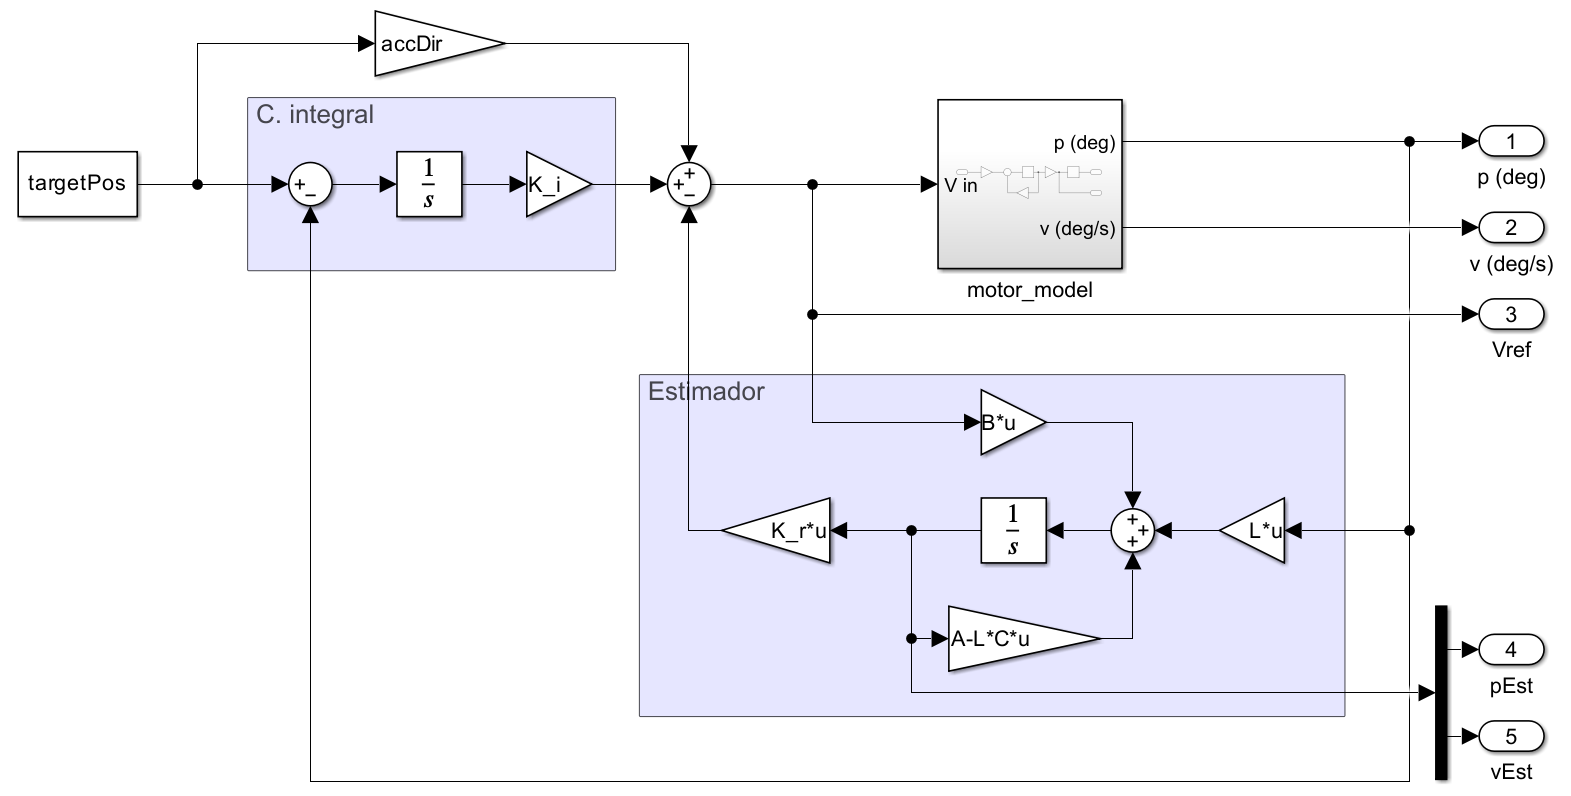
\includegraphics[width=0.75\linewidth]{img/controlador.png}
    \caption{Sistema del controlador con el motor ideal.}
    \label{fig:controlador}
\end{figure}

El modelo completo se presenta en la figura \ref{fig:controlador}. Para poder emplear el comando de \code{place} de MATLAB, se han elegido unos polos del estimador tal que $\lambda_e = \left[ -0.65, -0.6 \right]\cdot p$. El vector de polos aplicado a la matriz ampliada a la hora de calcular las ganancias de realimentación y control integral es $\lambda_{ri} = \left[ -0.3, -0.35, -0.4 \right]\cdot p$. Los resultados de simulación con estos polos se pueden ver en la figura \ref{fig:controlJusto}. En la figura se aprecia que se alcanza con éxito un valor de consigna de 5$\degree$. Lo que también se llega a apreciar sin problemas en la figura es el efecto que tiene la diferencia inicial entre el estimador y los estados reales. Esta diferencia provoca un pico en la acción del sistema, que se termina relajando según converge.

\begin{figure}[H]
    \centering
    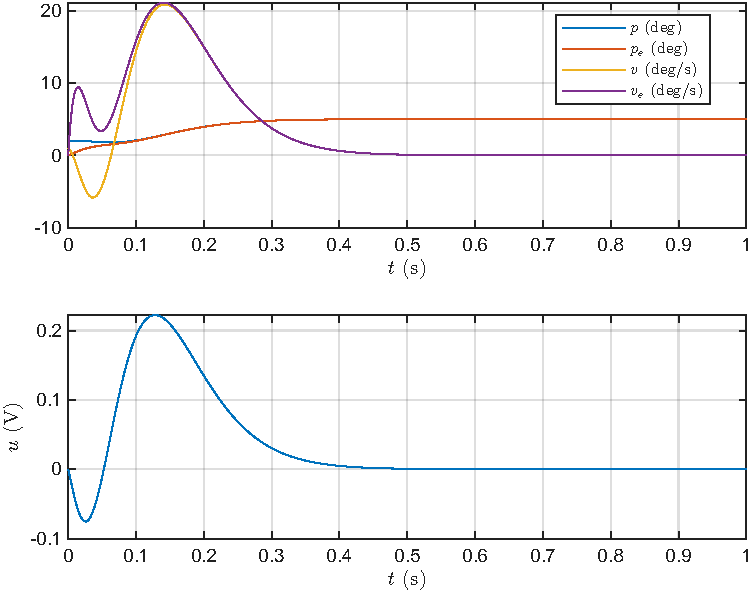
\includegraphics[width=0.75\linewidth]{img/controlJusto.pdf}
    \caption{Simulación con $\lambda_e = \left[ -0.65, -0.6 \right]\cdot p$ y $\lambda_{ri} = \left[ -0.3, -0.35, -0.4 \right]\cdot p$.}
    \label{fig:controlJusto}
\end{figure}

En las figuras a continuación (fig. \ref{fig:controlLento} y \ref{fig:controlRapido}) se observa el efecto que tiene en el sistema la colocación de los polos tanto del estimador como de la realimentación. En la figura \ref{fig:controlLento} se observa una respuesta lenta debido a unos polos mucho más pequeños. En este caso el sistema aporta todo el voltaje que puede para estabilizarlo, lo cual realmente no sería necesario si conociera la posición real. En la figura \ref{fig:controlRapido} se observa todo lo contrario, una respuesta muy rápida, que produce un pico de tensión muy alta también, y donde los estados llegan a tomar valores muy elevados. En el motor real, si la tensión de alimentación requerida supera 12 V únicamente lleva a una saturación y eventualmente alcanzará el valor deseado, por lo que lo ideal sería una respuesta más rápida que lenta.

\begin{figure}[H]
    \centering
    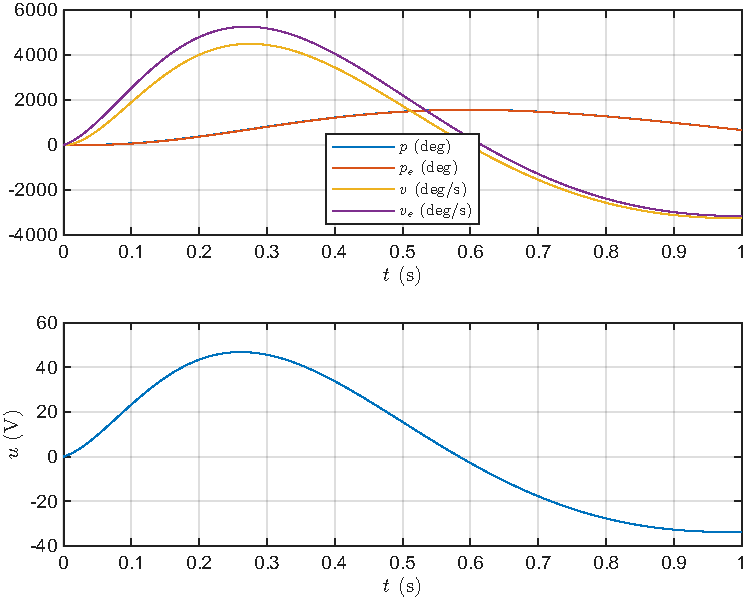
\includegraphics[width=0.75\linewidth]{img/controlLento.pdf}
    \caption{Simulación con $\lambda_e = \left[ -0.065, -0.06 \right]\cdot p$ y $\lambda_{ri} = \left[ -0.03, -0.035, -0.04 \right]\cdot p$.}
    \label{fig:controlLento}
\end{figure}

\begin{figure}[H]
    \centering
    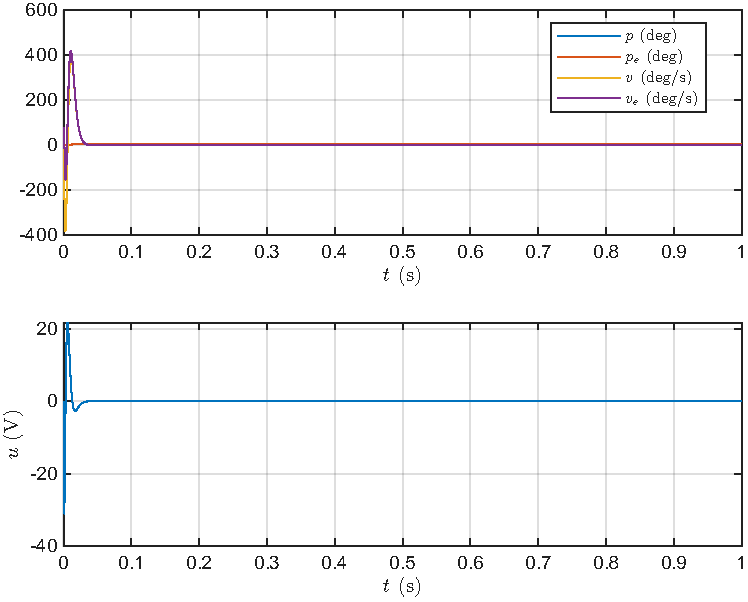
\includegraphics[width=0.75\linewidth]{img/controlRapido.pdf}
    \caption{Simulación con $\lambda_e = \left[ -65, -6 \right]\cdot p$ y $\lambda_{ri} = \left[ -3, -3.5, -4 \right]\cdot p$.}
    \label{fig:controlRapido}
\end{figure}

La ganancia denominada \code{accDir} es un remanente del control sin integrador. Si se ajusta esta ganancia sin presencia de un control integral, se puede forzar un valor de consigna manualmente. Pero como ya se ha mencionado, al estar empleando un control integral esta ganancia es innecesaria y se puede dejar 0. Ajustarla llevaría a un valor de
\begin{equation}
    F_c = \left[ -C\left[A-BK\right]^{-1}B \right]^{-1}.
\end{equation}

En la figura \ref{fig:accionDirecta} se puede observar una simulación con los mismos polos que la figura \ref{fig:controlJusto} y se aprecia como, pese a que el voltaje requerido es mayor, se alcanza la consigna más rápido.

\begin{figure}[H]
    \centering
    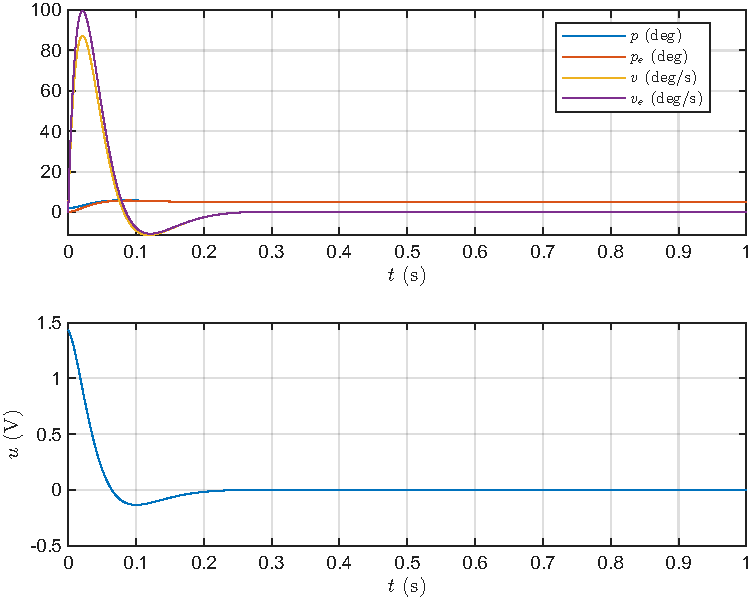
\includegraphics[width=0.75\linewidth]{img/accionDirecta.pdf}
    \caption{Simulación con la acción directa ajustada.}
    \label{fig:accionDirecta}
\end{figure}

\section{Discretización del controlador}

Para poder llegar a operar con el motor real se ha de tener en cuenta que todo se hace a través de un sistema digital: las operaciones no se hacen de modo continuo sino discreto. Es por esto que es necesario discretizar nuestro sistema. Para ello se empleará el bloque \textit{Zero-Order Hold} de Simulink. Este bloque muestrea las señales que le lleguen siguiendo un periodo proporcionado, el cual en este caso será $T = 0.1$ ms. Este periodo será el mismo que se emplea a la hora de simular el sistema, empleando pasos fijos de tamaño $T$. Sin embargo, al discretizar el sistema las matrices que lo describen son alteradas de tal manera que
\begin{equation}
    A \to F = \mathrm{e}^{AT};\quad B \to G = \mathrm{e}^{AT} \left[ \int^T_0 \mathrm{e}^{-\tau}\, \diff\tau \right] B.
\end{equation}

Gracias a estar usando MATLAB, no es necesario realizar ninguno de estos cálculos manualmente --programándolos, evidentemente--. Para hallar las nuevas matrices basta con definir un sistema continuo empleando la función \code{ss} y posteriormente crear la versión discretizada usando \code{c2d} pasando como argumentos el sistema continuo y el periodo $T$ elegido. Al haber cambiado las matrices del sistema también se han de recalcular los polos. La transformación de unos polos arbitrarios es 
\begin{equation}
    \lambda \to \Lambda = \mathrm{e}^{\lambda T},
\end{equation}
y finalmente el cálculo de ganancias de realimentación se realiza igual que en el sistema continuo, reemplazando adecuadamente las matrices y los polos.

Al igual que con el modelo en variables continuas, existe una ganancia de acción directa, $f$, para el sistema discretizado. Del mismo modo, realmente no es necesario ajustar esta ganancia debido a la acción integral de la cual se dispone. Sin embargo, se puede ajustar igualmente esta ganancia de la siguiente manera:
\begin{equation}
    f = \left[ C\left[ I-(F-GK) \right]^{-1}G \right]^{-1},
\end{equation}
la cual no siempre produce exactamente los mismos resultados que la ganancia $F_c$ si no fue ajustada. Para conseguir el mismo efecto en ambas, $f$ se puede alterar libremente para que su acción coincida con la del modelo continuo. Esto es gracias a la presencia de acción integral. Ahora $f$ toma el valor
\begin{equation}
    f = -\left[C\left[I-(F-GK) \right]^{-1}G\right]^{-1}C\left[A-BK\right]^{-1}BF_c.
\end{equation}

Simulando el sistema sin acción integral pero con la ganancia de acción directa ajustada se puede apreciar cómo el sistema también consigue alcanzar la consigna rápidamente (fig. \ref{fig:sinAccionIntegral}).

\begin{figure}[H]
    \centering
    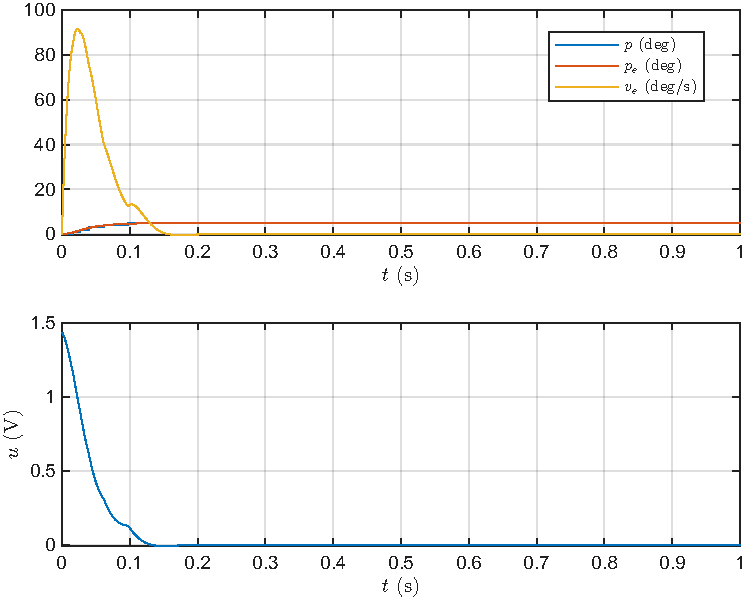
\includegraphics[width=0.75\linewidth]{img/sinAccionIntegral.pdf}
    \caption{Sistema simulado sin acción integral.}
    \label{fig:sinAccionIntegral}
\end{figure}

En la figura \ref{fig:accionDirectaDisc} se presenta la simulación correspondiente al valor ajustado de la acción directa. Comparando con la figura \ref{fig:controlJustoDisc}, con $f=0$, se observa cómo las diferencias son las mismas que para el control continuo. Salvando errores numéricos, la forma de la realimentación del sistema con acción directa es muy similar a la de la figura \ref{fig:accionDirecta}, tal y como se esperaba. En ambos sistemas se da una situación que previamente no se daba, que es que la posición estimada no termina de converger exactamente con la real, y además el voltaje suministrado no termina en 0, sino en un valor muy cercano. Esto es debido al bloque de \textit{deadzone} que se introdujo previamente para emular los voltajes bajos en los cuales el motor no tiene suficiente fuerza como para empezar a moverse.

\begin{figure}[H]
    \centering
    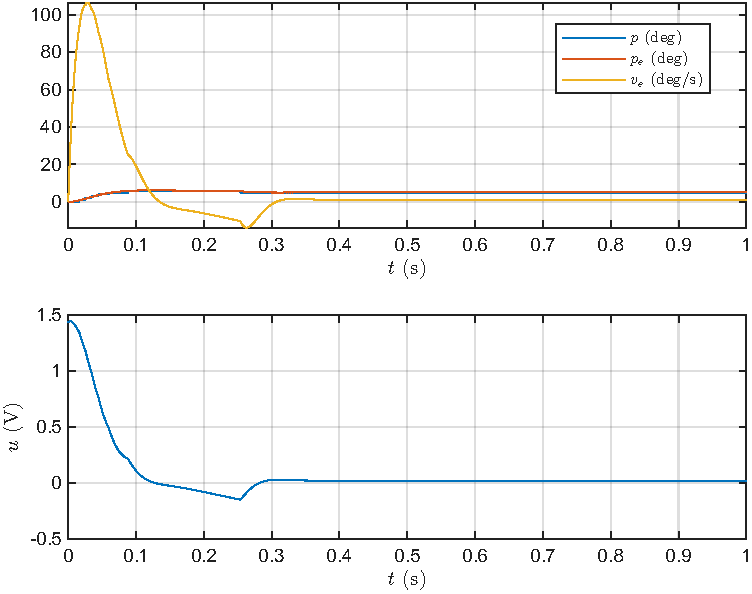
\includegraphics[width=0.75\linewidth]{img/accionDirectaDisc.pdf}
    \caption{Simulación con acción directa y polos discretizados para $\lambda_e = \left[ -0.65, -0.6 \right]\cdot p$ y $\lambda_{ri} = \left[ -0.3, -0.35, -0.4 \right]\cdot p$.}
    \label{fig:accionDirectaDisc}
\end{figure}

\begin{figure}[H]
    \centering
    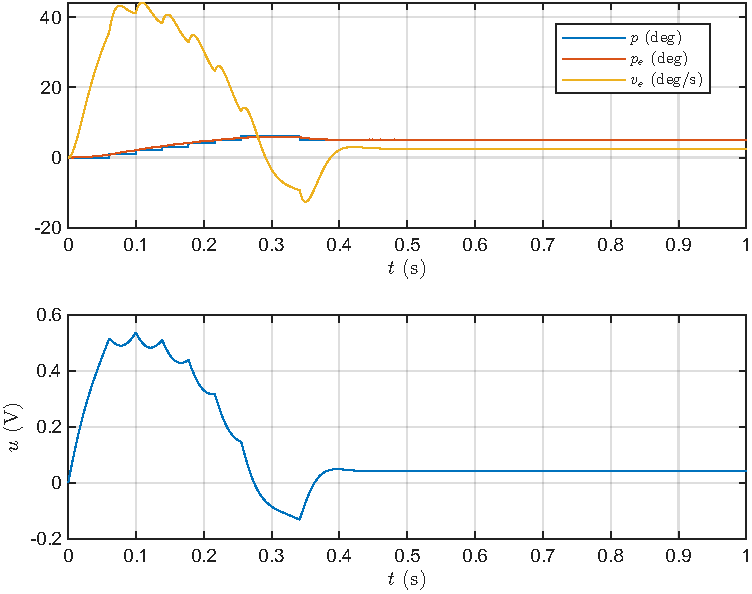
\includegraphics[width=0.75\linewidth]{img/controlJustoDisc.pdf}
    \caption{Simulación sin acción directa y polos discretizados para $\lambda_e = \left[ -0.65, -0.6 \right]\cdot p$ y $\lambda_{ri} = \left[ -0.3, -0.35, -0.4 \right]\cdot p$.}
    \label{fig:controlJustoDisc}
\end{figure}

Del mismo modo que para el sistema continuo, se puede forzar una respuesta muy rápida al sistema (fig. \ref{fig:controlRapidoDisc}) o una respuesta lenta (fig. \ref{fig:controlLentoDisc}).

\begin{figure}[H]
    \centering
    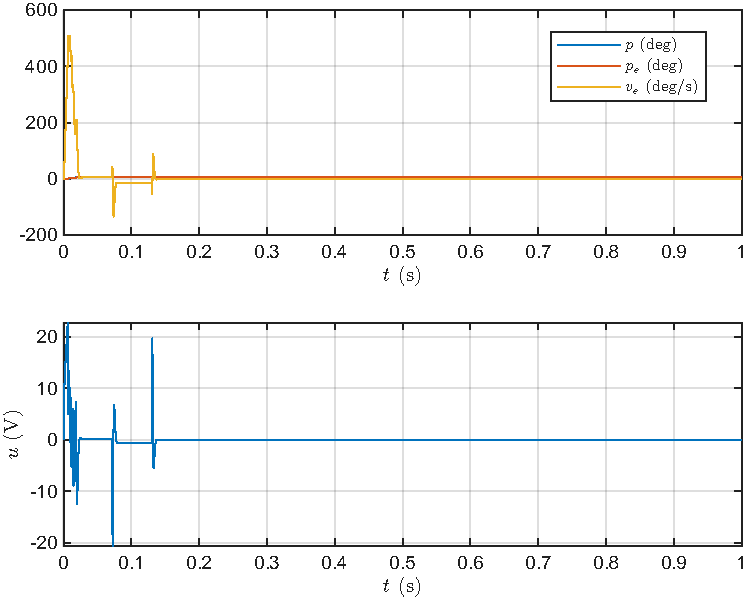
\includegraphics[width=0.75\linewidth]{img/controlRapidoDisc.pdf}
    \caption{Simulación sin acción directa y polos discretizados para $\lambda_e = \left[ -65, -6 \right]\cdot p$ y $\lambda_{ri} = \left[ -3, -3.5, -4 \right]\cdot p$.}
    \label{fig:controlRapidoDisc}
\end{figure}

\begin{figure}[H]
    \centering
    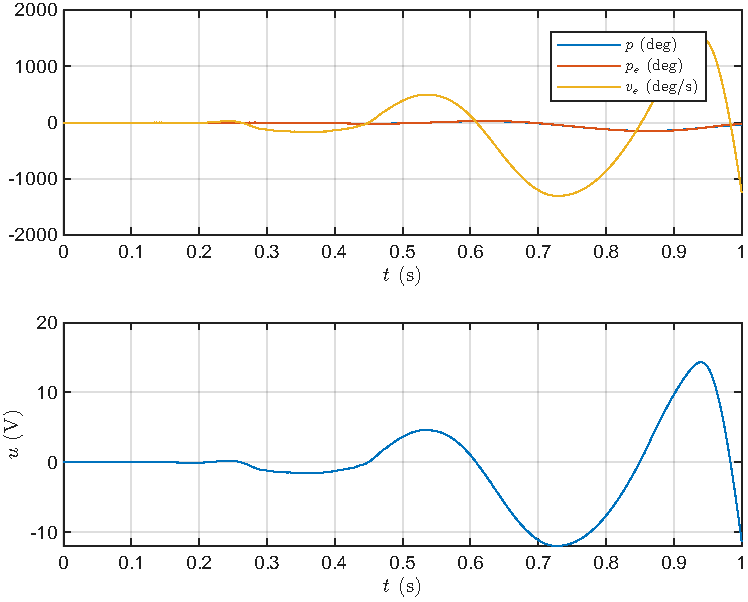
\includegraphics[width=0.75\linewidth]{img/controlLentoDisc.pdf}
    \caption{Simulación sin acción directa y polos discretizados para $\lambda_e = \left[ -0.065, -0.06 \right]\cdot p$ y $\lambda_{ri} = \left[ -0.03, -0.035, -0.04 \right]\cdot p$.}
    \label{fig:controlLentoDisc}
\end{figure}

Por último se añade al modelo un subsistema que intenta solucionar el problema del \textit{wind-up} --cuando la entrada al sistema satura--. El sistema completo se encuentra en la figura \ref{fig:controladorDisc}.

\begin{figure}[H]
    \centering
    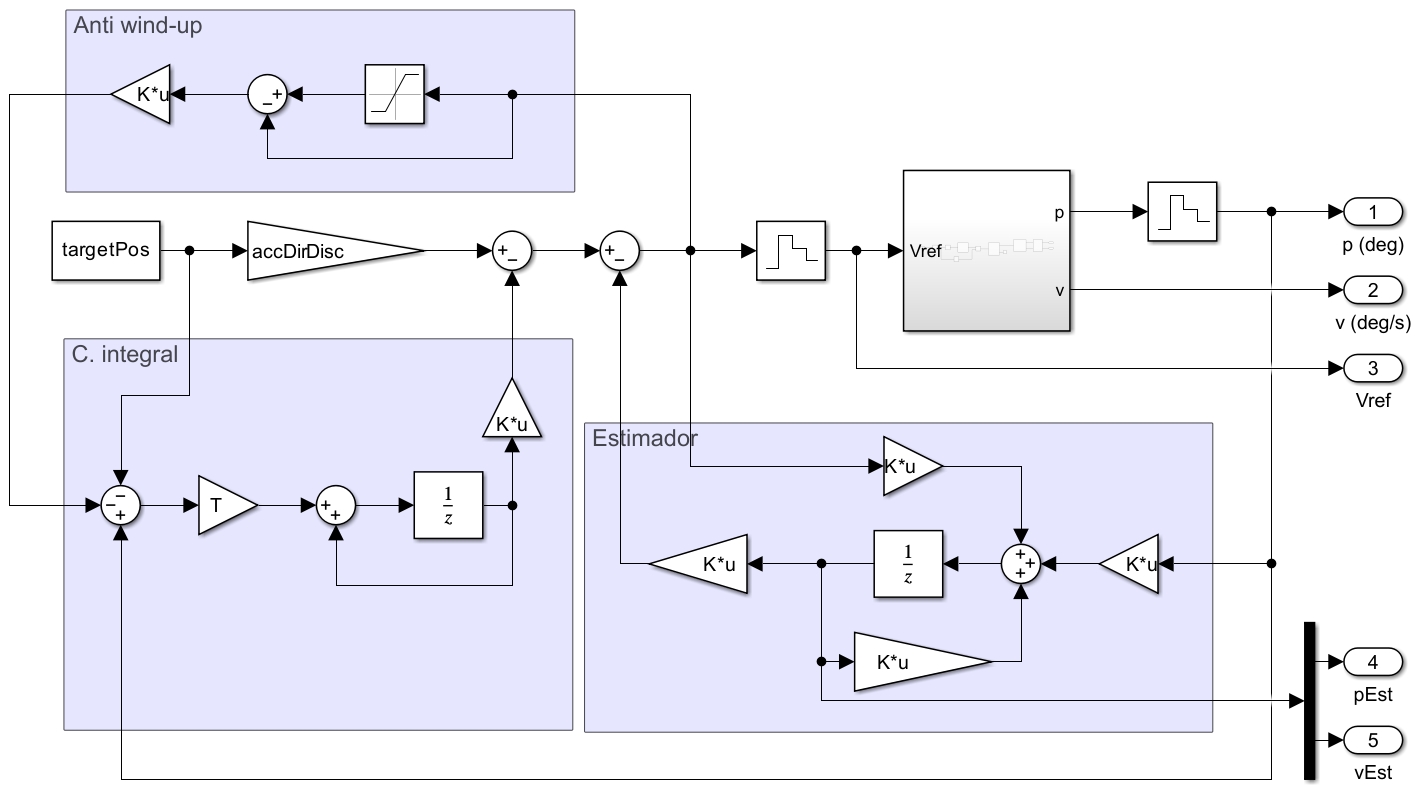
\includegraphics[width=0.75\linewidth]{img/controladorDisc.png}
    \caption{Sistema completo.}
    \label{fig:controladorDisc}
\end{figure}

Si se discretizan los polos situados en $\lambda_e = \left[ -5, -5.1 \right]\cdot p$ y $\lambda_{ri} = \left[ -4, -4.1, -4.2 \right]\cdot p$, se fuerza al sistema a saturar la señal pasados los 12 V. Con esto se puede comprobar el efecto que tiene la constante de anti \textit{wind-up} (fig. \ref{fig:antiWindUpFlojo}-\ref{fig:antiWindUpFuerte}). Se puede apreciar como para constantes demasiado altas se crean oscilaciones inducidas en la respuesta del sistema. Con esto se concluye que lo mejor es establecer la constante a un nivel relativamente bajo cercano a 0.1.

\begin{figure}[H]
    \centering
    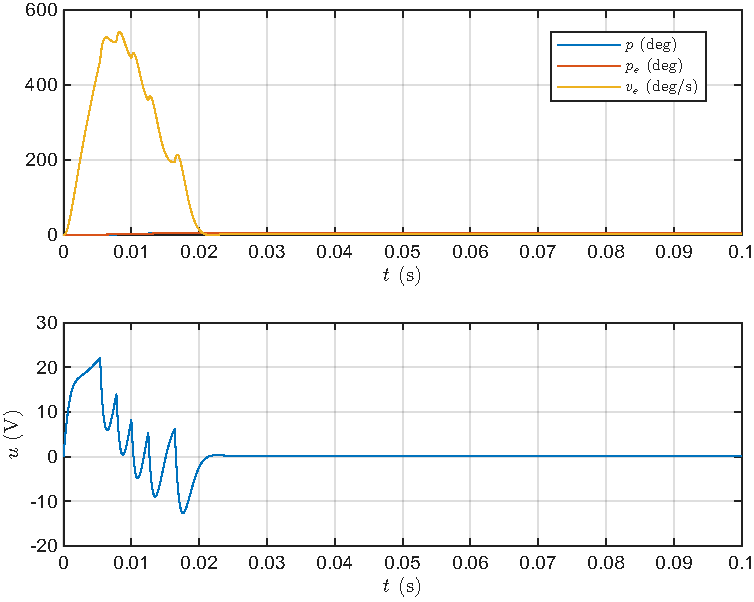
\includegraphics[width=0.75\linewidth]{img/antiWindUpFlojo.pdf}
    \caption{Anti \textit{wind-up} con $k = 0.1$.}
    \label{fig:antiWindUpFlojo}
\end{figure}

\begin{figure}[H]
    \centering
    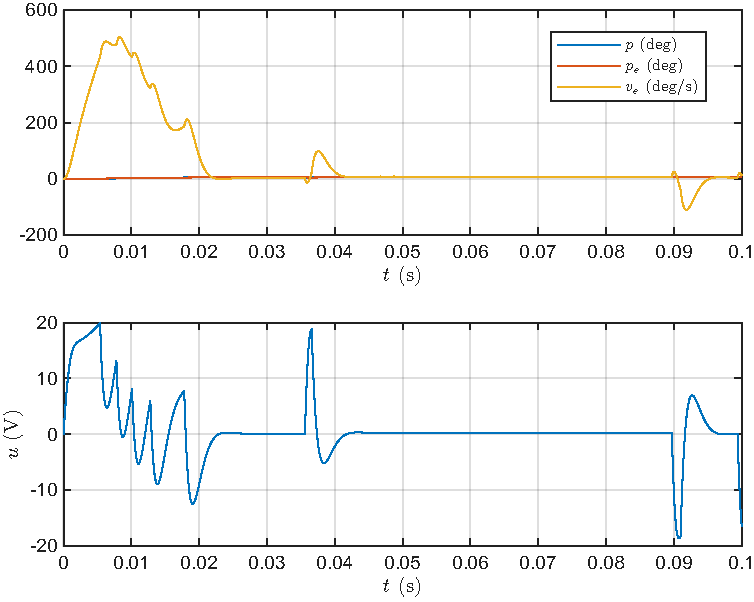
\includegraphics[width=0.75\linewidth]{img/antiWindUpMedio.pdf}
    \caption{Anti \textit{wind-up} con $k = 0.2$.}
    \label{fig:antiWindUpMedio}
\end{figure}

\begin{figure}[H]
    \centering
    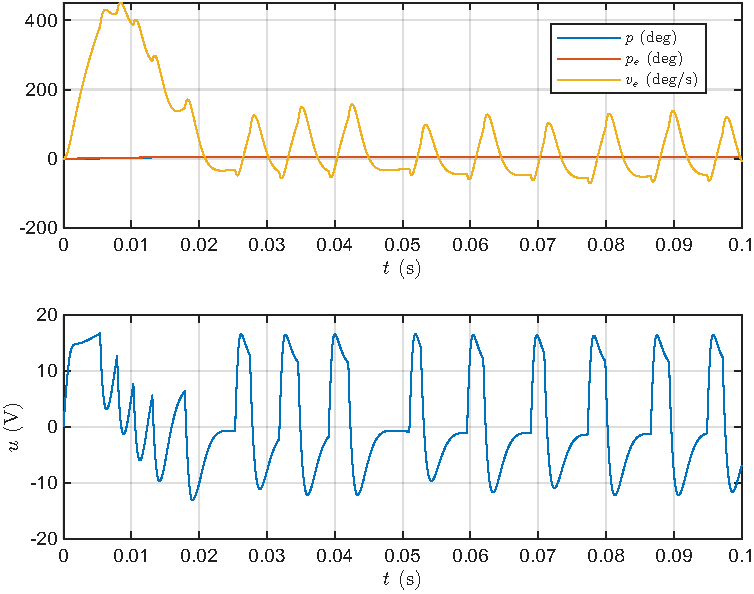
\includegraphics[width=0.75\linewidth]{img/antiWindUpFuerte.pdf}
    \caption{Anti \textit{wind-up} con $k = 0.5$.}
    \label{fig:antiWindUpFuerte}
\end{figure}


\section{Acción sobre el motor real}

Con el controlador discreto terminado, queda sustituir el modelo del motor (fig \ref{fig:simIdeal}) del controlador de la figura \ref{fig:controladorDisc} por el motor real (fig. \ref{fig:modeloLazoAbierto}). Además, es importante añadir un par de bloques más a la entrada del motor real. Éste toma señales de entrada normalizadas a 100, de manera que 12 V sea equivalente a 100. Esto se arregla con una ganancia de $\frac{100}{12}$. Además, hay que especificar el sentido de giro por separado del valor de la señal, de manera que se toma el valor absoluto para la señal, y el sentido de giro se determina con una comparación con 0. Estos cambios se pueden ver reflejados en la figura \ref{fig:controladorReal}.

\begin{figure}[H]
    \centering
    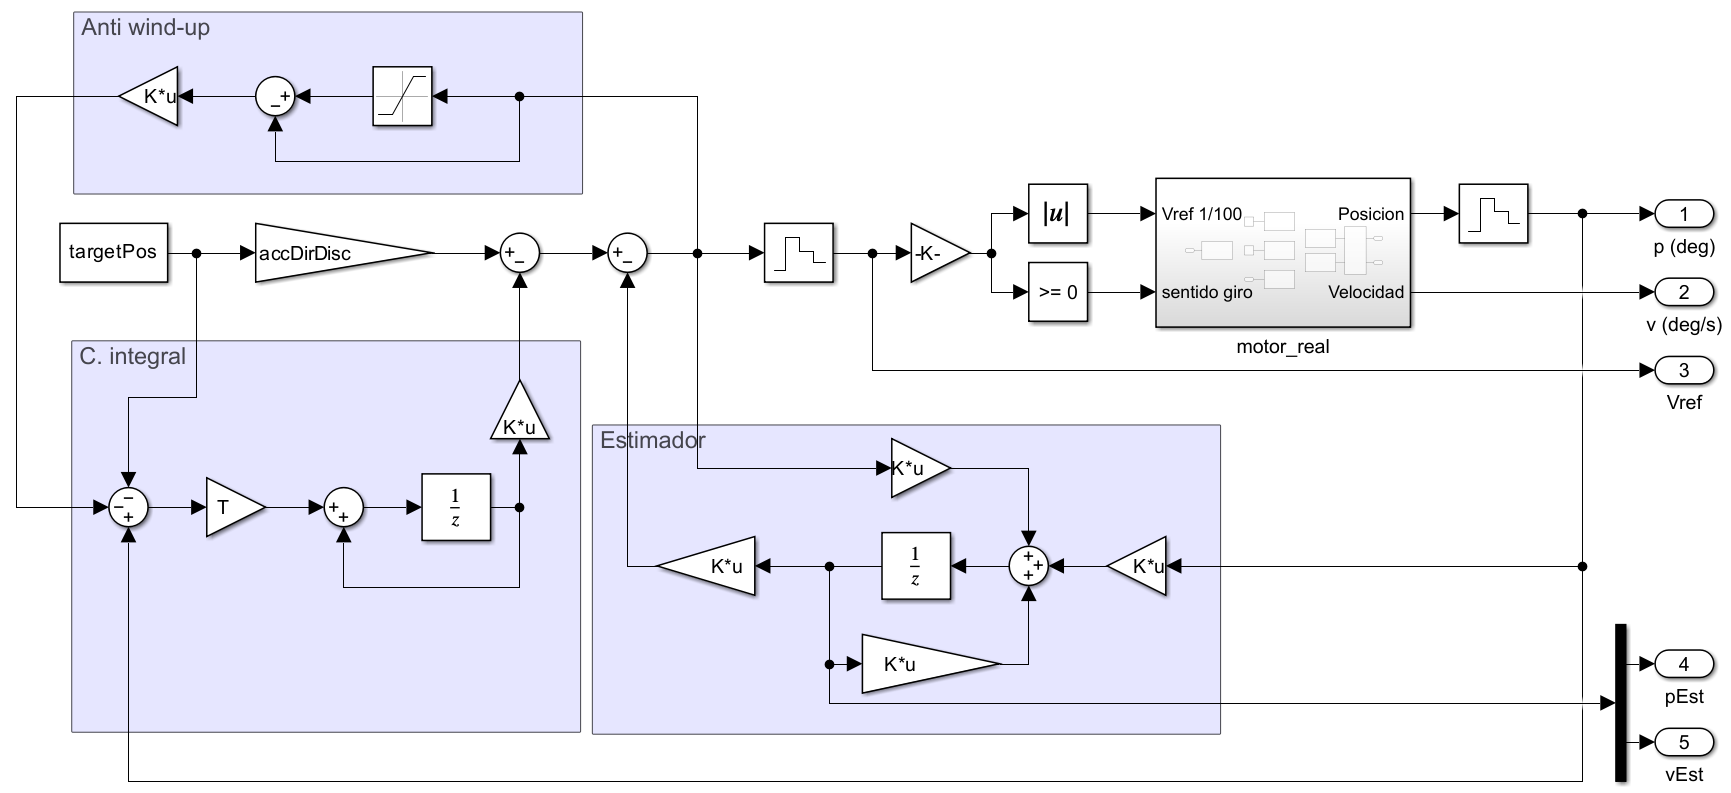
\includegraphics[width=0.75\linewidth]{img/controladorReal.png}
    \caption{Controlador con el motor real implementado.}
    \label{fig:controladorReal}
\end{figure}

Finalmente ya están listos todos los preparativos para realizar medidas y aplicar el controlador en el motor real. Para comprobar el correcto funcionamiento de todos los subsistemas, se selecciona una consigna de $\pm180\degree$. En las figuras \ref{fig:controlRealPos} y \ref{fig:controlRealNeg} se pueden ver los resultados del controlador. Tal y como se esperaba, se alcanza la consigna perfectamente. Además, se puede apreciar cómo la señal de entrada se satura, pasando los 12 V, y se activa el anti \textit{wind-up}. Como se predijo, la saturación del sistema no le evite eventualmente alcanzar la consigna determinada. Además, se observa cómo el sentido de giro se transmite correctamente, alcanzando la consigna con el signo adecuado.

\begin{figure}[H]
    \centering
    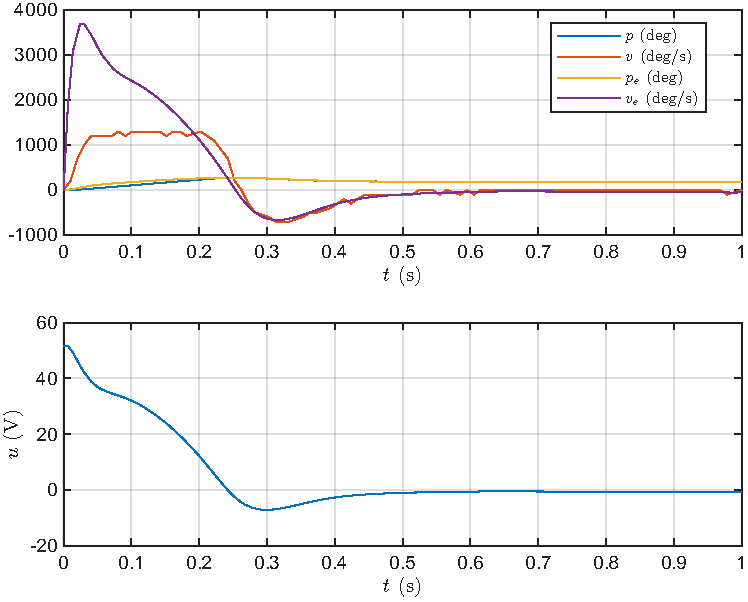
\includegraphics[width=0.75\linewidth]{img/controlRealPos.pdf}
    \caption{Control real del motor con una consigna positiva de 180$\degree$.}
    \label{fig:controlRealPos}
\end{figure}

\begin{figure}[H]
    \centering
    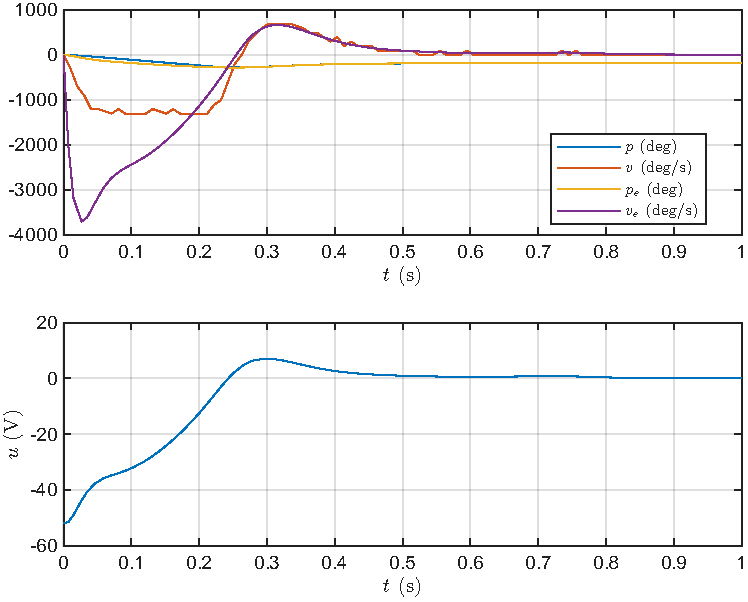
\includegraphics[width=0.75\linewidth]{img/controlRealNeg.pdf}
    \caption{Control real del motor con una consigna negativa de -180$\degree$.}
    \label{fig:controlRealNeg}
\end{figure}

\section*{Anexo I}

El código empleado se presenta a continuación, y también está disponible en el siguiente repositorio de GitHub: \url{https://github.com/n0rbb/Realimentados/tree/cambios-miguel/practica_motor/realizacion}.

\begin{minted}[mathescape, linenos, bgcolor=light-gray]{MATLAB}
% Cargamos los datos medidos
motor_data = load('motor_data\all_data.mat')

% Posiciones
figure
hold on
for i = 1:12
    % Extracción de datos
    % Los archivos tienen el formato motorXXV, siendo XX el voltage
    % suministrado al motor
    voltage = pad(num2str(i), 2, "left", '0');
    extracted = motor_data.(strcat('motor',voltage,'V')).getElement('Motor:1');
    positions = extracted.Values.Data;
    time = extracted.Values.Time;
    % Representación
    plot(time, positions, DisplayName=strcat(voltage,'V'))
    grid on
end
legend(Location="northwest")
xlabel('$t$ (s)', Interpreter='latex')
ylabel('$p$ (deg)', Interpreter='latex')
exportgraphics(gcf,'figuras\posicionLazoAbierto.pdf')

% Velocidades
figure
hold on
for i = 1:12
    % Extracción de datos
    voltage = pad(num2str(i), 2, "left", '0');
    extracted = motor_data.(strcat('motor',voltage,'V')).getElement('Motor:2');
    positions = extracted.Values.Data;
    time = extracted.Values.Time;
    % Representación
    plot(time, positions, DisplayName=strcat(voltage,'V'))
    grid on
end
legend(Location="northwest")
xlabel('$t$ (s)', Interpreter='latex')
ylabel('$v$ (deg/s)', Interpreter='latex')
xlim([0 5])
exportgraphics(gcf,'figuras\velocidadLazoAbierto.pdf')

% Comprobación de encoders
encoder_data = load('motor_data\encoders_raw.mat')
encoderA = encoder_data.data.getElement('Encoder A:1').Values.Data;
timeA = encoder_data.data.getElement('Encoder A:1').Values.Time;
encoderB = encoder_data.data.getElement('Encoder B:1').Values.Data;
timeB = encoder_data.data.getElement('Encoder B:1').Values.Time;
figure
plot(timeA, encoderA(:), DisplayName='Enconder A')
hold on
plot(timeB, encoderB(:), DisplayName='Enconder B')
grid on
legend
xlim([1 1.1])
xlabel('$t$ (s)', Interpreter='latex')
exportgraphics(gcf,'figuras\encodersCheck.pdf')


% Modelado
syms V k_e p t
angularPos = V*k_e/p^2*exp(-p*t) + V*k_e/p*t - V*k_e/p^2
angularVel = diff(angularPos,t)

% Identificación - cargado de datos
motor_data = load('motor_data\all_data.mat')

% Ajuste lineal de los datos
% Se preasignan los tamaños de las variables
lin_fit = ones([12 2]);
ke_mat = ones([12 1]);
p_mat = ones([12 1]);
for i = 1:12
    % Extracción de datos
    voltage = pad(num2str(i), 2, "left", '0');
    extracted = motor_data.(strcat('motor',voltage,'V')).getElement('Motor:1');
    positions = extracted.Values.Data(401:1200); % sólo 2s del motor encendido
    time = extracted.Values.Time(1:800); % tiempos re-centrados en 0
    % Ajuste lineal.
    lin_fit(i,:) = polyfit(time, positions, 1);
    ke_mat(i) = -lin_fit(i,1)^2 / (lin_fit(i,2) * i);
    p_mat(i) = -lin_fit(i,1) / lin_fit(i,2);
end
% Los parámetros del sistema serán
ke_mat, p_mat
ke = mean(ke_mat)
p = mean(p_mat)
% Construimos las matrices del sistema
A = [0 1; 0 -p]
B = [0 ke]'
C = [1 0]
D = 0;

% Comprobación
open('motor_ideal.slx')
figure(1)
clf
hold on
figure(2)
clf
hold on
for i = 1:12
    voltage = i;
    simOut = sim('motor_ideal.slx');
    time = simOut.tout;
    angPos = simOut.yout{1}.Values.Data;
    angVel = simOut.yout{2}.Values.Data;
    figure(1)
    plot(time, angPos, DisplayName=strcat(num2str(voltage),'V'))
    figure(2)
    plot(time, angVel, DisplayName=strcat(num2str(voltage),'V'))
end
figure(1)
grid on
legend(Location="northwest")
xlabel('$t$ (s)', Interpreter='latex')
ylabel('$x$ (deg)', Interpreter='latex')
xlim([0 5])
exportgraphics(gcf,'figuras\posicionIdeal.pdf')
figure(2)
grid on
legend(Location="northwest")
xlabel('$t$ (s)', Interpreter='latex')
ylabel('$v$ (deg/s)', Interpreter='latex')
xlim([0 5])
exportgraphics(gcf,'figuras\velocidadIdeal.pdf')


% Simulación ideal
% Definición de parámetros para la simulación
tPWM = 1e-3;
Vmax = 12;

% Comprobación de encoders
voltage = 6;
tf = 1;
stepTime = 0;
open('simIdeal.slx')
simOut = sim('simIdeal.slx');
timeReal = simOut.tout;
timePos = simOut.yout{1}.Values.Time;
angPos = simOut.yout{1}.Values.Data;
timeVel = simOut.yout{2}.Values.Time;
angVel = simOut.yout{2}.Values.Data;
angPosReal = simOut.yout{3}.Values.Data;
angVelReal = simOut.yout{4}.Values.Data;
figure
subplot(2,1,1)
plot(timePos,angPos)
hold on
plot(timeReal,angPosReal)
grid on
legend('Lectura de encoder','Posición real',Location="northwest")
xlabel('$t$ (s)', Interpreter='latex')
ylabel('$x$ (deg)', Interpreter='latex')
xlim([0 1])
subplot(2,1,2)
plot(timeVel,angVel)
hold on
plot(timeReal,angVelReal)
grid on
legend('Lectura de encoder','Velocidad real',Location="southeast")
xlabel('$t$ (s)', Interpreter='latex')
ylabel('$v$ (deg/s)', Interpreter='latex')
xlim([0 1])
exportgraphics(gcf,'figuras\comprobacionEncoders.pdf')

% Comparación con los datos reales
tf = 5;
stepTime = 1;
figure(27)
clf
hold on
figure(34)
clf
hold on
for i = 1:12
    voltage = i;
    simOut = sim('simIdeal.slx');
    timePos = simOut.yout{1}.Values.Time;
    angPos = simOut.yout{1}.Values.Data;
    timeVel = simOut.yout{2}.Values.Time;
    angVel = simOut.yout{2}.Values.Data;
    figure(27)
    plot(timePos, angPos, DisplayName=strcat(num2str(voltage),'V'))
    figure(34)
    plot(timeVel, angVel, DisplayName=strcat(num2str(voltage),'V'))
end
figure(27)
grid on
legend(Location="northwest")
xlabel('$t$ (s)', Interpreter='latex')
ylabel('$x$ (deg)', Interpreter='latex')
xlim([0 5])
exportgraphics(gcf,'figuras\posicionIdealEncoder.pdf')
figure(34)
grid on
legend(Location="northwest")
xlabel('$t$ (s)', Interpreter='latex')
ylabel('$v$ (deg/s)', Interpreter='latex')
xlim([0 5])
exportgraphics(gcf,'figuras\velocidadIdealEncoder.pdf')


% Ganancia del estimador
poles_e = [-0.65*p -0.6*p];
L = place(A',C',poles_e)';
% Ganancias de realimentación de estados y del control integral
A_ri = [A zeros(2,1); C 0];
B_ri = [B; 0];
poles_ri = [-0.3*p -0.35*p -0.4*p];
K_ri = place(A_ri,B_ri,poles_ri);
K_r = K_ri(1:2);
K_i = K_ri(3);
% Condiciones inciales del sistema
p0 = 2;
v0 = 1;
accDir = (-C*(A-B*K_r)^-1*B)^-1;
% Posición de consigna
targetPos = 5;

% Se simula con la acción directa correcta
open('controller.slx')
simOut = sim('controller.slx');
time = simOut.tout;
angPos = simOut.yout{1}.Values.Data;
angVel = simOut.yout{2}.Values.Data;
voltage = simOut.yout{3}.Values.Data;
angPosEst = simOut.yout{4}.Values.Data;
angVelEst = simOut.yout{5}.Values.Data;
figure
subplot(2,1,1)
plot(time,angPos)
hold on
plot(time,angPosEst)
plot(time,angVel)
plot(time,angVelEst)
grid on
legend('$p$ (deg)','$p_e$ (deg)','$v$ (deg/s)','$v_e$ (deg/s)', ...
    Location="best", Interpreter='latex')
xlabel('$t$ (s)', Interpreter='latex')
xlim([0 1])
subplot(2,1,2)
plot(time,voltage)
grid on
xlabel('$t$ (s)', Interpreter='latex')
ylabel('$u$ (V)', Interpreter='latex')
xlim([0 1])
exportgraphics(gcf,'figuras\accionDirecta.pdf')

% Se simula el sistema para diferentes polos
accDir = 0;
simOut = sim('controller.slx');
time = simOut.tout;
angPos = simOut.yout{1}.Values.Data;
angVel = simOut.yout{2}.Values.Data;
voltage = simOut.yout{3}.Values.Data;
angPosEst = simOut.yout{4}.Values.Data;
angVelEst = simOut.yout{5}.Values.Data;
figure
subplot(2,1,1)
plot(time,angPos)
hold on
plot(time,angPosEst)
plot(time,angVel)
plot(time,angVelEst)
grid on
legend('$p$ (deg)','$p_e$ (deg)','$v$ (deg/s)','$v_e$ (deg/s)', ...
    Location="best", Interpreter='latex')
xlabel('$t$ (s)', Interpreter='latex')
xlim([0 1])
subplot(2,1,2)
plot(time,voltage)
grid on
xlabel('$t$ (s)', Interpreter='latex')
ylabel('$u$ (V)', Interpreter='latex')
xlim([0 1])
exportgraphics(gcf,'figuras\controlJusto.pdf')

poles_e = [-0.065*p -0.06*p];
L = place(A',C',poles_e)';
poles_ri = [-0.03*p -0.035*p -0.04*p];
K_ri = place(A_ri,B_ri,poles_ri);
K_r = K_ri(1:2);
K_i = K_ri(3);
simOut = sim('controller.slx');
time = simOut.tout;
angPos = simOut.yout{1}.Values.Data;
angVel = simOut.yout{2}.Values.Data;
voltage = simOut.yout{3}.Values.Data;
angPosEst = simOut.yout{4}.Values.Data;
angVelEst = simOut.yout{5}.Values.Data;
figure
subplot(2,1,1)
plot(time,angPos)
hold on
plot(time,angPosEst)
plot(time,angVel)
plot(time,angVelEst)
grid on
legend('$p$ (deg)','$p_e$ (deg)','$v$ (deg/s)','$v_e$ (deg/s)', ...
    Location="best", Interpreter='latex')
xlabel('$t$ (s)', Interpreter='latex')
xlim([0 1])
subplot(2,1,2)
plot(time,voltage)
grid on
xlabel('$t$ (s)', Interpreter='latex')
ylabel('$u$ (V)', Interpreter='latex')
xlim([0 1])
exportgraphics(gcf,'figuras\controlLento.pdf')

poles_e = [-6.5*p -6*p];
L = place(A',C',poles_e)';
poles_ri = [-3*p -3.5*p -4*p];
K_ri = place(A_ri,B_ri,poles_ri);
K_r = K_ri(1:2);
K_i = K_ri(3);
simOut = sim('controller.slx');
time = simOut.tout;
angPos = simOut.yout{1}.Values.Data;
angVel = simOut.yout{2}.Values.Data;
voltage = simOut.yout{3}.Values.Data;
angPosEst = simOut.yout{4}.Values.Data;
angVelEst = simOut.yout{5}.Values.Data;
figure
subplot(2,1,1)
plot(time,angPos)
hold on
plot(time,angPosEst)
plot(time,angVel)
plot(time,angVelEst)
grid on
legend('$p$ (deg)','$p_e$ (deg)','$v$ (deg/s)','$v_e$ (deg/s)', ...
    Location="best", Interpreter='latex')
xlabel('$t$ (s)', Interpreter='latex')
xlim([0 1])
subplot(2,1,2)
plot(time,voltage)
grid on
xlabel('$t$ (s)', Interpreter='latex')
ylabel('$u$ (V)', Interpreter='latex')
xlim([0 1])
exportgraphics(gcf,'figuras\controlRapido.pdf')


% Discretizamos el sistema continuo
motorCont = ss(A,B,C,D);
T = 1e-4;
motorDisc = c2d(motorCont,T);
F = motorDisc.A;
G = motorDisc.B;
% Recalculamos los polos de la realimentación, el integrador y el estimador
F_ri = [F zeros(2,1); T*C 1];
G_ri = [G; 0];
poles_ri_disc = exp([-0.3*p -0.35*p -0.4*p]*T);
K_ri_disc = place(F_ri,G_ri,poles_ri_disc);
K_r_disc = K_ri_disc(1:2);
K_i_disc = K_ri_disc(3);
poles_e_disc = exp([-0.65*p -0.6*p]*T);
L_disc = place(F',C',poles_e_disc)';

% Constantes
k_awp = 0.1;
accDirDisc = ( C*( (eye(2)-(F-G*K_r_disc))^-1 * G ) )^-1;
accInt = 1;

% Se simula con la acción directa correcta y acción integral
open('controller_disc.slx')
simOut = sim('controller_disc.slx');
time = simOut.tout;
angPos = simOut.yout{1}.Values.Data;
voltage = simOut.yout{3}.Values.Data;
angPosEst = simOut.yout{4}.Values.Data;
angVelEst = simOut.yout{5}.Values.Data;
figure
subplot(2,1,1)
plot(time,angPos)
hold on
plot(time,angPosEst)
plot(time,angVelEst)
grid on
legend('$p$ (deg)','$p_e$ (deg)','$v_e$ (deg/s)', ...
    Location="best", Interpreter='latex')
xlabel('$t$ (s)', Interpreter='latex')
xlim([0 1])
subplot(2,1,2)
plot(time,voltage)
grid on
xlabel('$t$ (s)', Interpreter='latex')
ylabel('$u$ (V)', Interpreter='latex')
xlim([0 1])
exportgraphics(gcf,'figuras\accionDirectaDisc.pdf')

% Sin acción integral
accInt = 0;
simOut = sim('controller_disc.slx');
time = simOut.tout;
angPos = simOut.yout{1}.Values.Data;
voltage = simOut.yout{3}.Values.Data;
angPosEst = simOut.yout{4}.Values.Data;
angVelEst = simOut.yout{5}.Values.Data;
figure
subplot(2,1,1)
plot(time,angPos)
hold on
plot(time,angPosEst)
plot(time,angVelEst)
grid on
legend('$p$ (deg)','$p_e$ (deg)','$v_e$ (deg/s)', ...
    Location="best", Interpreter='latex')
xlabel('$t$ (s)', Interpreter='latex')
xlim([0 1])
subplot(2,1,2)
plot(time,voltage)
grid on
xlabel('$t$ (s)', Interpreter='latex')
ylabel('$u$ (V)', Interpreter='latex')
xlim([0 1])
exportgraphics(gcf,'figuras\sinAccionIntegral.pdf')

% Se simula el sistema para diferentes polos
accDirDisc = 0;
accInt = 1;
simOut = sim('controller_disc.slx');
time = simOut.tout;
angPos = simOut.yout{1}.Values.Data;
voltage = simOut.yout{3}.Values.Data;
angPosEst = simOut.yout{4}.Values.Data;
angVelEst = simOut.yout{5}.Values.Data;
figure
subplot(2,1,1)
plot(time,angPos)
hold on
plot(time,angPosEst)
plot(time,angVelEst)
grid on
legend('$p$ (deg)','$p_e$ (deg)','$v_e$ (deg/s)', ...
    Location="best", Interpreter='latex')
xlabel('$t$ (s)', Interpreter='latex')
xlim([0 1])
subplot(2,1,2)
plot(time,voltage)
grid on
xlabel('$t$ (s)', Interpreter='latex')
ylabel('$u$ (V)', Interpreter='latex')
xlim([0 1])
exportgraphics(gcf,'figuras\controlJustoDisc.pdf')

poles_ri_disc = exp([-0.03*p -0.035*p -0.04*p]*T);
K_ri_disc = place(F_ri,G_ri,poles_ri_disc);
K_r_disc = K_ri_disc(1:2);
K_i_disc = K_ri_disc(3);
poles_e_disc = exp([-0.065*p -0.06*p]*T);
L_disc = place(F',C',poles_e_disc)';
simOut = sim('controller_disc.slx');
time = simOut.tout;
angPos = simOut.yout{1}.Values.Data;
voltage = simOut.yout{3}.Values.Data;
angPosEst = simOut.yout{4}.Values.Data;
angVelEst = simOut.yout{5}.Values.Data;
figure
subplot(2,1,1)
plot(time,angPos)
hold on
plot(time,angPosEst)
plot(time,angVelEst)
grid on
legend('$p$ (deg)','$p_e$ (deg)','$v_e$ (deg/s)', ...
    Location="best", Interpreter='latex')
xlabel('$t$ (s)', Interpreter='latex')
xlim([0 1])
subplot(2,1,2)
plot(time,voltage)
grid on
xlabel('$t$ (s)', Interpreter='latex')
ylabel('$u$ (V)', Interpreter='latex')
xlim([0 1])
exportgraphics(gcf,'figuras\controlLentoDisc.pdf')

poles_ri_disc = exp([-3*p -3.5*p -4*p]*T);
K_ri_disc = place(F_ri,G_ri,poles_ri_disc);
K_r_disc = K_ri_disc(1:2);
K_i_disc = K_ri_disc(3);
poles_e_disc = exp([-6.5*p -6*p]*T);
L_disc = place(F',C',poles_e_disc)';
simOut = sim('controller_disc.slx');
time = simOut.tout;
angPos = simOut.yout{1}.Values.Data;
voltage = simOut.yout{3}.Values.Data;
angPosEst = simOut.yout{4}.Values.Data;
angVelEst = simOut.yout{5}.Values.Data;
figure
subplot(2,1,1)
plot(time,angPos)
hold on
plot(time,angPosEst)
plot(time,angVelEst)
grid on
legend('$p$ (deg)','$p_e$ (deg)','$v_e$ (deg/s)', ...
    Location="best", Interpreter='latex')
xlabel('$t$ (s)', Interpreter='latex')
xlim([0 1])
subplot(2,1,2)
plot(time,voltage)
grid on
xlabel('$t$ (s)', Interpreter='latex')
ylabel('$u$ (V)', Interpreter='latex')
xlim([0 1])
exportgraphics(gcf,'figuras\controlRapidoDisc.pdf')

% Con diferentes constantes de anti wind-up
poles_ri_disc = exp([-4*p -4.1*p -4.2*p]*T);
K_ri_disc = place(F_ri,G_ri,poles_ri_disc);
K_r_disc = K_ri_disc(1:2);
K_i_disc = K_ri_disc(3);
poles_e_disc = exp([-5*p -5.1*p]*T);
L_disc = place(F',C',poles_e_disc)';
accInt = 1;
accDirDisc = 0;
k_awp = 0.1;
simOut = sim('controller_disc.slx');
time = simOut.tout;
angPos = simOut.yout{1}.Values.Data;
voltage = simOut.yout{3}.Values.Data;
angPosEst = simOut.yout{4}.Values.Data;
angVelEst = simOut.yout{5}.Values.Data;
figure
subplot(2,1,1)
plot(time,angPos)
hold on
plot(time,angPosEst)
plot(time,angVelEst)
grid on
legend('$p$ (deg)','$p_e$ (deg)','$v_e$ (deg/s)', ...
    Location="best", Interpreter='latex')
xlabel('$t$ (s)', Interpreter='latex')
xlim([0 0.1])
subplot(2,1,2)
plot(time,voltage)
grid on
xlabel('$t$ (s)', Interpreter='latex')
ylabel('$u$ (V)', Interpreter='latex')
xlim([0 0.1])
exportgraphics(gcf,'figuras\antiWindUpFlojo.pdf')

k_awp = 0.2;
simOut = sim('controller_disc.slx');
time = simOut.tout;
angPos = simOut.yout{1}.Values.Data;
voltage = simOut.yout{3}.Values.Data;
angPosEst = simOut.yout{4}.Values.Data;
angVelEst = simOut.yout{5}.Values.Data;
figure
subplot(2,1,1)
plot(time,angPos)
hold on
plot(time,angPosEst)
plot(time,angVelEst)
grid on
legend('$p$ (deg)','$p_e$ (deg)','$v_e$ (deg/s)', ...
    Location="best", Interpreter='latex')
xlabel('$t$ (s)', Interpreter='latex')
xlim([0 0.1])
subplot(2,1,2)
plot(time,voltage)
grid on
xlabel('$t$ (s)', Interpreter='latex')
ylabel('$u$ (V)', Interpreter='latex')
xlim([0 0.1])
exportgraphics(gcf,'figuras\antiWindUpMedio.pdf')

k_awp = 0.5;
simOut = sim('controller_disc.slx');
time = simOut.tout;
angPos = simOut.yout{1}.Values.Data;
voltage = simOut.yout{3}.Values.Data;
angPosEst = simOut.yout{4}.Values.Data;
angVelEst = simOut.yout{5}.Values.Data;
figure
subplot(2,1,1)
plot(time,angPos)
hold on
plot(time,angPosEst)
plot(time,angVelEst)
grid on
legend('$p$ (deg)','$p_e$ (deg)','$v_e$ (deg/s)', ...
    Location="best", Interpreter='latex')
xlabel('$t$ (s)', Interpreter='latex')
xlim([0 0.1])
subplot(2,1,2)
plot(time,voltage)
grid on
xlabel('$t$ (s)', Interpreter='latex')
ylabel('$u$ (V)', Interpreter='latex')
xlim([0 0.1])
exportgraphics(gcf,'figuras\antiWindUpFuerte.pdf')


% Con consigna positiva
data_pos = load('motor_data\motor_real_control.mat')
p = data_pos.data.getElement('p (deg):1').Values.Data;
pTime = data_pos.data.getElement('p (deg):1').Values.Time;
v = data_pos.data.getElement('v (deg//s):1').Values.Data;
vTime = data_pos.data.getElement('v (deg//s):1').Values.Time;
pEst = data_pos.data.getElement('pEst:1').Values.Data;
pEstTime = data_pos.data.getElement('pEst:1').Values.Time;
vEst = data_pos.data.getElement('vEst:1').Values.Data;
vEstTime = data_pos.data.getElement('vEst:1').Values.Time;
Vref = data_pos.data.getElement('Vref:1').Values.Data;
VrefTime = data_pos.data.getElement('Vref:1').Values.Time;
% Representación
figure
subplot(2,1,1)
plot(pTime,p)
hold on
plot(vTime,v)
plot(pEstTime,pEst)
plot(vEstTime,vEst)
grid on
legend('$p$ (deg)','$v$ (deg/s)','$p_e$ (deg)','$v_e$ (deg/s)', ...
    Location="best", Interpreter='latex')
xlabel('$t$ (s)', Interpreter='latex')
xlim([0 1])
subplot(2,1,2)
plot(VrefTime,Vref)
grid on
xlabel('$t$ (s)', Interpreter='latex')
ylabel('$u$ (V)', Interpreter='latex')
xlim([0 1])
exportgraphics(gcf,'figuras\controlRealPos.pdf')

% Con consigna negativa
data_neg = load('motor_data\motor_real_control_neg.mat')
p = data_neg.data.getElement('p (deg):1').Values.Data;
pTime = data_neg.data.getElement('p (deg):1').Values.Time;
v = data_neg.data.getElement('v (deg//s):1').Values.Data;
vTime = data_neg.data.getElement('v (deg//s):1').Values.Time;
pEst = data_neg.data.getElement('pEst:1').Values.Data;
pEstTime = data_neg.data.getElement('pEst:1').Values.Time;
vEst = data_neg.data.getElement('vEst:1').Values.Data;
vEstTime = data_neg.data.getElement('vEst:1').Values.Time;
Vref = data_neg.data.getElement('Vref:1').Values.Data;
VrefTime = data_neg.data.getElement('Vref:1').Values.Time;
% Representación
figure
subplot(2,1,1)
plot(pTime,p)
hold on
plot(vTime,v)
plot(pEstTime,pEst)
plot(vEstTime,vEst)
grid on
legend('$p$ (deg)','$v$ (deg/s)','$p_e$ (deg)','$v_e$ (deg/s)', ...
    Location="best", Interpreter='latex')
xlabel('$t$ (s)', Interpreter='latex')
xlim([0 1])
subplot(2,1,2)
plot(VrefTime,Vref)
grid on
xlabel('$t$ (s)', Interpreter='latex')
ylabel('$u$ (V)', Interpreter='latex')
xlim([0 1])
exportgraphics(gcf,'figuras\controlRealNeg.pdf')
\end{minted}


%---------------------------------------------------

\end{document}